% !TEX encoding = UTF-8
% !TEX TS-program = pdflatex
% !TEX root = ../Appunti.tex

\section{Gas ideale}
\label{sec:idgas}

Le definizioni di gas perfetto e ideale sono state date nel primo capitolo, e sono rispettivamente la \cref{def:perfgas} e la \cref{def:idgas}.

Si ricorda che la condizione di idealità era data da:
\begin{equation*}
e^{\mu/k_B T} \ll 1
\end{equation*}

Calcolando il valore del numero di particelle per mezzo della densità di stati:
\begin{equation*}
N = \sum_{\textbf{q}} \overline{n_{\textbf{q}}} = \int \exp \left(- \frac{\varepsilon - \mu}{k_B T}\right) \rho(\varepsilon) \dd \varepsilon = \frac{V}{\Lambda^3} e^{\mu/k_B T}
\end{equation*}
\begin{equation*}
\Lambda = \frac{2\pi \hbar}{\sqrt{2\pi m k_B T}}
\end{equation*}
dove si sta imponendo la condizione di idealità, assumendo, nel calcolo di $ \overline{n_{\textbf{q}}} $, che ci sia al più una particella per microstato.

Per cui la condizione di idealità può essere riespressa in funzione della densità $\rho$ del sistema:
\begin{equation*}
	e^{\mu/k_B T} = \Lambda^3 \frac{N}{V} = \Lambda^3 \rho	\qquad \implies \qquad \rho \ll \frac{1}{\Lambda^3}
\end{equation*}
Si può interpretare $ \Lambda^3 \rho $ come la frazione di volume occupata dal gas (cioè $ \Lambda^3 $ come il volume della particella).

Per cui $\Lambda(T)$ fornisce il parametro su cui valutare l'idealità del gas, e dipende dalla temperatura $T$ del sistema, perciò è detta \textit{lunghezza d'onda termica} di De Broglie.

Essa è detta lunghezza d'onda perché si può immaginare di raccogliere le onde piane in pacchetti localizzati, e l'ordine di grandezza sarebbe quello di $\Lambda$, infatti per il principio di indeterminazione la minima indeterminazione possibile sarà proporzionale a $\hbar/p$, ma $p$ tipico sarà determinato dall'energia, che è quella termica, per cui $p \sim (2 m k_B T)^{1/2}$.

Per cui $\Lambda^3$ è la dimensione tipica dei pacchetti d'onda, e la condizione di idealità corrisponde quindi a richiedere che i pacchetti risultino puntiformi rispetto alle distanze tipiche del sistema, in modo che gli effetti quantistici non siano coinvolti nella dinamica.

Si possono inoltre ricavare le altre proprietà del gas ideale a partire dalla energia libera di Gibbs:
\begin{align*}
	\mu &= - k_B T \log \frac{k_B T}{P \Lambda^3}\\
	G &= N\mu = - N k_B T \log \frac{k_B T}{P \Lambda^3}
\end{align*}

In particolare per l'entropia e le due capacità termiche:
\begin{align*}
	S &= -Nk_B \log \frac{N}{V} + \frac{3}{2} N k_B \log k_B T + N k_B \left(\frac{5}{2} + \frac{3}{2}\log \frac{m}{2\pi \hbar^2}\right)\\
	C_P &= \frac{5}{2} N k_B \qquad C_V = \frac{3}{2} N k_B
\end{align*}

Nel precedente capitolo le proprietà del gas perfetto erano state discusse usando l'approccio canonico, e quindi ricavandosi l'energia libera $F$:
\begin{equation*}
	F_c = - N k_B T \log \left(\frac{V}{\Lambda^3}\right) + k_B T \log N!
\end{equation*}

Il problema è che l'energia libera, calcolata a partire dall'energia libera ricavata nell'approccio grancanonico, è apparentemente differente:
\begin{equation*}
F_{gc} = G - PV = - N k_B T \log \left(\frac{V}{N \Lambda^3}\right) - N k_B T
\end{equation*}

\noindent Per cui:
\begin{equation*}
	F_{gc} - F_c = k_B T (N \log N - N - \log N!)
\end{equation*}
ma questa differenza si annulla asintoticamente con $N \rightarrow \infty$, per l'approssimazione di Stirling. 
Questo risultato era prevedebile: nell'approccio canonico il sistema ha un numero di particelle fissato, mentre nell'approccio grancanonico il numero di particelle può fluttuare, ma le fluttuazioni relative si annullano asintoticamente.

\begin{ex}[Approssimazione di Stirling]
	L'approssimazione di Stirling si può ricavare sviluppando $\log N!$ in forma di serie, e approssimandolo con un integrale su un supporto opportuno.
\end{ex}

\paragraph{Deviazioni dall'idealità} Si nota che la questione di un gas perfetto e non ideale è apparentemente del tutto teorica. Infatti le tipiche condizioni sotto cui un gas è perfetto sono le stesse sotto cui è ideale:
\begin{description}
	\item[bassa densità] in modo tale che la distanza tra le particelle sia grande rispetto alla scala tipica dell'interazione (nel caso dell'idealità il confronto era da farsi con la scala di lunghezza data dall'indeterminazione quantistica);
	\item[alta temperatura] l'energia delle interazioni dev'essere piccola rispetto all'altra scala di energia: l'energia termica (nel caso dell'idealità la temperatura entra in gioco nel determinare le scale di lunghezza).
\end{description}

Per cui tipicamente quando vengono meno le condizioni di idealità vengono meno anche quelle di perfezione. Anzi, spesso la condizione di gas non interagente è la prima ad essere violata (la scala dell'indeterminazione quantistica è più piccola di quella delle interazioni).

In realtà sono noti esempi in cui il gas si comporta come non ideale, anche se le interazioni continuano a non essere sostanzialmente rilevanti (elettroni in un metallo tipicamente, o in parte è anche il caso delle stelle di neutroni, in cui però sono coinvolti effetti relativi alla gravità).

Per il momento si procede semplicemente studiando la questione.

\section{Statistiche di Bose-Einstein e Fermi-Dirac}
\label{sec:BFstat}

In meccanica quantistica l'\textit{identicità} delle particelle ha un significato molto più forte che in meccanica classica: essa è strettamente correlata al \textit{principio di indeterminazione}.

Infatti l'identificazione di una particella implica la localizzazione nello spazio fisico, ma questo porta a una grande indeterminazione sull'impulso, che comporta che tale identificazione venga persa subito dopo. In altri termini: mentre in meccanica classica le particelle potevano essere identiche, ma data una configurazione iniziale era possibile \textit{seguire le traiettorie} e riconoscere a un dato istante che una data particella fosse quella che era partita in un dato punto, questa possibilità si perde in meccanica quantistica.
\newline

\`E noto, dalla meccanica quantistica, che il modo corretto di trattare le particelle identiche è quello di assegnare al sistema a molti-corpi funzioni d'onda che siano \textit{completamente simmetriche o antisimmetriche} per scambio di particelle.

In particolare: 
\begin{itemize}
	\item se le funzioni d'onda possono essere solo completamente simmetriche, cioè invarianti per permutazioni, le particelle vengono dette \textit{bosoni}, e si distribuiscono secondo la statistica di Bose-Einstein;
	\item se le funzioni d'onda possono essere solo completamente antisimmetriche, cioè sotto permutazione vengono moltiplicate per il segno di essa ($-1$ per le dispari, $1$ per le pari), vengono dette \textit{fermioni}, e soddisfano la statistica di Fermi-Dirac.
\end{itemize}

L'effetto dei due vincoli è quello di consentire, per ogni stato di singola particella, tutti i possibili \textit{numeri d'occupazione} nel caso dei bosoni, mentre esclusivamente $0,1$ per i fermioni (infatti se ci fosse più di una particella nello stesso stato scambiandone due si troverebbe che la funzione d'onda è pari a meno se stessa, e quindi nulla).
\newline

Si considera quindi il caso di un gas perfetto nei due scenari descritti.

Si noti che le probabilità di occupazione di uno stato di singola particella in un gas perfetto sono note dalla generalizzazione dell'ensemble di Gibbs al caso grancanonico, e sono:
\begin{equation*}
w_{\textbf{q},n} = \exp \left[-\frac{(\varepsilon_{\textbf{q}} - \mu) n_{\textbf{q}}}{k_B T}\right]
\end{equation*}
\textit{indipendentemente} dalle considerazioni sull'\textit{identicità} delle particelle.

\subsection{Fermi-Dirac}

Si esamina il comportamento del gas perfetto applicando il metodo suggerito in \cref{sec:idpart}: lo studio dei numeri di occupazione degli stati di singola particella.
La funzione di granpartizione del singolo stato è dunque:
\begin{equation*}
\Omega_{\textbf{q}} = - k_B T \log \left[1 + \exp \left(-\frac{\varepsilon_{\textbf{q}} - \mu}{k_B T}\right)\right]
\end{equation*}
poiché l'antisimmetrizzazione delle funzioni d'onda esclude la presenza di più particelle nello stesso stato, quindi i numeri di occupazione maggiori di $1$, e di conseguenza la somma è troncata.

Questo risultato è formalmente identico a quello trovato nel caso di particelle classiche, ma vi è una differenza sostanziale è \textit{esatto}. 
Infatti nel caso classico era il risultato di una approssimazione, e quindi aveva dei limiti sulla validità.

Questo fatto garantisce il corretto limite classico, nel caso in cui le condizioni dell'approssimazione precedente siano nuovamente verificate.
\newline

Studiando il numero di occupazione medio del singolo stato, si ottiene:
\begin{equation*}
\overline{n_{\textbf{q}}} = - \partdev{\Omega_{\textbf{q}}}{\mu} = \frac{\exp\left[(\varepsilon_{\textbf{q}} - \mu)/k_B T\right]}{1 + \exp\left[(\varepsilon_{\textbf{q}} - \mu)/k_B T\right]} = \frac{1}{\exp\left[(\varepsilon_{\textbf{q}} - \mu)/k_B T\right] + 1}
\end{equation*}
per cui il numero medio di occupazione è sempre minore di $1$ (nel limite classico $\ll 1$).

Per ottenere l'intera funzione di granpartizione e il numero di particelle si sommano le precedenti quantità su tutti gli stati possibili.

\subsection{Bose-Einstein}
Si applica lo stesso metodo descritto nel caso precedente, però vengono meno i vincoli imposti dall'antisimettrizzazione (la funzione d'onda è simmetrica anche se tutte le particelle sono nello stesso stato, anzi, lo è in modo naturale).

La funzione di granpartizione del singolo stato è dunque:
\begin{equation*}
\Omega_{\textbf{q}} = - k_B T \log \left[\sum_{n_{\textbf{q}}=0}^{N} \exp \left(-\frac{(\varepsilon_{\textbf{q}} - \mu )n_{\textbf{q}}}{k_B T}\right)\right] \simeq - k_B T \log \left[\sum_{n_{\textbf{q}}=0}^{\infty} \exp \left(-\frac{(\varepsilon_{\textbf{q}} - \mu) n_{\textbf{q}}}{k_B T}\right)\right]
\end{equation*}
Si nota che l'approssimazione considerata non è altro che il limite termodinamico, inoltre è ben verificata anche per $N$ finiti, infatti la probabilità $w_{\textbf{q}}$ è comunque soppressa esponenzialmente con il numero di occupazione.

Si è approssimato con una serie perché essa è una serie geometrica \footnotemark, e quindi si sa calcolare esattamente, e si trova:
\begin{equation*}
\Omega_{\textbf{q}} = - k_B T \log \left[\frac{1}{1 - \exp[-(\varepsilon_{\textbf{q}} - \mu)/k_B T]}\right] = k_B T \log \left[1 - \exp(-\frac{\varepsilon_{\textbf{q}} - \mu}{k_B T})\right]
\end{equation*}

Perché la serie non diverga è necessario però che:
\begin{equation*}
\mu < \varepsilon_{\textbf{q}} ~~\forall \textbf{q} \qquad \iff \qquad \mu < \varepsilon_0
\end{equation*}
dove si è indicato con $\varepsilon_0$ l'energia del fondamentale. Nel caso di un gas perfetto in cui il volume in cui è contenuto è molto più grande rispetto alla scala della lunghezza d'onda termica l'energia del fondamentale è trascurabile, per cui si richiede $\mu < 0$.
\footnotetext{Se ci fosse bisogno di ricordarlo:
\begin{equation*}
\sum_{n=0}^{\infty} x^n = \frac{1}{1-x}
\end{equation*}
}

Studiando il numero di occupazione medio del singolo stato, si ottiene:
\begin{equation*}
\overline{n_{\textbf{q}}} = - \partdev{\Omega_{\textbf{q}}}{\mu} = \frac{1}{ \exp\left[(\varepsilon_{\textbf{q}} - \mu)/k_B T\right] - 1}
\end{equation*}
si noti che in questo caso non ci sono limiti al numero di occupazione possibile.

Come nel caso del gas di Fermi per ottenere l'intera funzione di partizione o il numero di particelle si somma su tutti gli stati possibili.

Anche in questo caso nel limite di alte temperature e basse densità si recupera il caso classico; infatti espandendo il $\log$ in $\Omega_{\textbf{q}}$ si recupera il segno di differenza dal caso del gas di Fermi, e quindi coincidendo col gas di Fermi coincide col caso classico.

\section{Gas poco degenere}
\label{sec:fewdegas}

\subsubsection{Integrazione sugli stati}
\`E ancora possibile integrare sugli stati, anziché sommare, nelle condizioni in cui si presentano effetti quantistici rilevanti?

\noindent La risposta è quasi sempre sì. Non è vero per ogni regime, ma le condizioni che portano a commettere un grosso errore effetuando l'integrazione sono ancora più stringenti di quelle che portano al manifestarsi della natura quantistica della materia.

Infatti il criterio per valutare l'errore commesso nell'integrazione si basa su quanto siano ravvicinati gli stati, cioè se la differenza in energia tra gli stati (detta in inglese \textit{energy gap}) sia molto minore della scale energetiche di interesse del problema.

In particolare confrontando tale differenza con l'energia termica si ottiene la condizione:
\begin{equation*}
	\frac{\hbar^2}{2m}\left(\frac{2\pi}{L}\right)^2 \ll \kt
\end{equation*}
dove $L$ è la scala tipica delle dimensioni lineari del sistema (che al limite termodinamico $ \rightarrow \infty $).

\begin{es}
Per dare un'idea degli ordini di grandezza in gioco nel caso di $L \sim \unit{1}{\centi\meter}$ e $m \sim \unit{10^{-24}}{\gram}$ - l'ordine di grandezza della massa dell'atomo di idrogeno - si ha che la temperatura fissata dall'\textit{energy gap} è pari a $\sim \unit{10^{-13}}{\kelvin}$. Se invece si usa la massa dell'elettrone $m \sim \unit{10^{-27}}{\gram}$ si ottiene una temperatura $\sim \unit{10^{-10}}{\kelvin}$.
In entrambi i casi sono limiti facilmente rispettati.
\end{es}

\subsubsection{Correzioni al caso classico}

\paragraph{Degenerazione di spin} C'è un ulteriore considerazione da fare, legata ai gradi di libertà di \textit{spin}. Nel caso più semplice in assenza di campo (che è quello che si andrà qui a considerare) l'effetto è quelo di inserire una degenerazione ulteriore nei livelli energetici:
\begin{equation*}
g = 2S + 1
\end{equation*}
per cui lo spazio delle fasi diventa:
\begin{equation*}
g \frac{\dd ^3 p \dd ^3 r}{(2\pi \hbar)^3}
\end{equation*}
e anche nella densità di stati compare quindi il fattore $g$.

In seguito tale fattore sarà considerato $g=1$ per i bosoni e $g=2$ per i fermioni, in quanto il caso tipico di applicazione saranno fermioni di spin $1/2$ o bosoni a spin nullo.

\paragraph{Equazione di stato} Si procede esaminando l'insorgere di effetti quantistici in un gas classico che comincia ad allontanarsi dal regime di idealità. Per fare ciò si espandano al secondo ordine nella condizione di idealità $e^{\mu/k_B T} \ll 1$ le espressioni trovate per $\Omega$\footnote{Il segno superiore si riferisce a Fermi-Dirac, quello inferiore a Bose-Einstein}:
\begin{align*}
	\Omega &\simeq \mp \sum_{\textbf{q}} \log(1 \pm \exp[-\frac{\varepsilon_{\textbf{q}} - \mu}{k_B T}]) = -k_B T \sum_{\textbf{q}} \exp(-\frac{\varepsilon_{\textbf{q}} - \mu}{k_B T}) \pm \frac{k_B T}{2} \sum_{\textbf{q}} \exp(-2\frac{(\varepsilon_{\textbf{q}} - \mu)}{k_B T}) = \\
	&= \Omega_{class} \pm \frac{k_B T}{2} \exp(\frac{2\mu}{k_B T})\sum_{\textbf{q}} \exp(-\frac{2\varepsilon_{\textbf{q}} }{k_B T})
\end{align*}
dove $\Omega_{class}$ è la funzione di granpartizione classica, che come detto nella \cref{sec:BFstat} costituisce il prim'ordine della funzione di granpartizione in entrambi i casi quantistici.

Si deve quindi valutare la somma, e in accordo a quanto detto prima lo si fa integrando:
\begin{equation*}
\sum_{\textbf{q}} \exp(-\frac{2\varepsilon_{\textbf{q}} }{k_B T}) \simeq \int_0^{\infty} \rho(\varepsilon) \exp(-\frac{2\varepsilon }{k_B T}) \dd \varepsilon = \left(\frac{1}{2}\right)^{3/2 } \int_0^{\infty} \rho(2\varepsilon) \exp(-\frac{2\varepsilon }{k_B T}) \dd (2\varepsilon)
\end{equation*}
dove si è usato il fatto che $\rho(\varepsilon) \propto \varepsilon^{1/2}$, per cui la correzione è:
\begin{equation*}
\pm \left(\frac{1}{2}\right)^{5/2}k_B T e^{2\mu/k_B T}  \int_0^{\infty} \rho(\varepsilon) \exp(-\frac{\varepsilon }{k_B T}) \dd \varepsilon
\end{equation*}
mentre il termine dominante è:
\begin{equation*}
\Omega_{class} = -k_B T \sum_{\textbf{q}} \exp(-\frac{\varepsilon_{\textbf{q}} - \mu}{k_B T}) \simeq - k_B T e^{\mu/k_B T}  \int_0^{\infty} \rho(\varepsilon) \exp(-\frac{\varepsilon }{k_B T}) \dd \varepsilon
\end{equation*}

Si ottiene infine:
\begin{equation*}
	\Omega \simeq \Omega_{class}\left[1 \mp \frac{e^{\mu/k_B T}}{2^{5/2}}\right]
\end{equation*}
e quindi, considerando che $\Omega = - PV$ e $\Omega_{class} = - N k_B T$, l'equazione di stato è:
\begin{equation*}
	PV = N k_B T \left[1 \mp \frac{e^{\mu/k_B T}}{2^{5/2}}\right]
\end{equation*}

Per interpretare tale correzione si deve considerare il procedimento utilizzato: usando $\Omega$ si è considerato l'approccio grancanonico, in cui $T,V$ e $\mu$ sono fissati, ma $N$ è libero. Per cui la correzione trovata non è direttamente una correzione alla pressione, ma una correzione a $P/N$.

\noindent Per capire cosa stia succedendo al gas è più facile chiedersi cosa accade alla pressione se $T,V$ e $N$ sono costanti, in modo da trovare esplicitamente la nuova pressione, così da confrontarla col caso classico.

Per raggiungere questo obiettivo è naturale passare per l'energia libera $F$, dato che sono le sue variabili proprie.
Si ha dalla \cref{sec:thermquant}:
\begin{equation*}
(\delta \Omega)_{T, V, \mu} = (\delta F)_{T,V,N}
\end{equation*}
e usando la notazione:
\begin{align*}
\Omega(T,V,\mu) &= \Omega_{class} + (\delta \Omega)_{T, V, \mu}\\
F(T,V,N) &= F_{class} + (\delta F)_{T, V, N}
\end{align*}
si ha:
\begin{equation*}
\delta \Omega = \mp \Omega_{class}\frac{e^{\mu/k_B T}}{2^{5/2}} = \pm N k_B T \frac{e^{\mu/k_B T}}{2^{5/2}}
\end{equation*}

Per trovare la correzione a $F$ si deve esprimere $\mu$ nell'espressione precedente in funzione di $T,V,N$. Si sostituisce il valore:
\begin{equation*}
\mu_{class} = -k_B T \log\frac{V}{N \Lambda^3}
\end{equation*}
in quanto includendo in $\mu$ qualunque correzione, già a partire dal prim'ordine, si otterebbero correzioni di ordine superiore al primo nella pressione.

Si trova quindi per $F$:
\begin{equation*}
F = F_{class} \pm \frac{N^2 k_B T \Lambda^3}{2^{5/2} V}
\end{equation*}
e infine per la pressione:
\begin{equation*}
P = - \partdev{F}{V} = P_{class} \pm \frac{N^2 k_B T \Lambda^3}{2^{5/2} V^2} = \frac{N k_B T}{V} \left(1  \pm \frac{N\Lambda^3}{2^{5/2} V}\right)
\end{equation*}

Come atteso le correzioni sono piccole nella quantità $\Lambda^3 \rho = N\Lambda^3 / V$, che evidenziano come gli effetti quantistici derivino dall'\textit{overlap} del supporto dei pacchetti d'onda delle particelle.

Osservando il segno delle correzioni si nota che:
\begin{itemize}
	\item per il \textbf{gas di Fermi} il \textit{principio di esclusione di Pauli} agisce come una sorta di forza repulsiva, aumentando la pressione del gas rispetto al caso classico;
	\item per il \textbf{gas di Bose} l'assenza di restrizioni agisce come una interazione attrattiva fra le particelle, diminuendo la pressione.
\end{itemize}

\section{Gas di Fermi molto degenere: elettroni nei metalli}
\label{sec:fermigas}
La descrizione del comportamento degli elettroni nei metalli, e quindi delle peculiari proprietà che distinguono i metalli dagli altri elementi, è uno dei grandi successi della teoria del gas di Fermi degenere.
\newline

Si esamina quindi cosa succede ai fermioni nel limite opposto a quello classico, cioè il limite di bassa temperatura.
Lo stato "asintotico" è relativamente facile da esaminare: si impone $T=0$, e quindi che il sistema stia nel fondamentale, esattamente.

La struttura del fondamentale a molti corpi è piuttosto semplice: si comincia a riempire gli stati di singola particella a partire dal fondamentale e salendo via via, scegliendo sempre quello a più bassa energia disponibile, fino a esaurimento delle particelle. Per particelle di spin $S$ si deve ricordare di considerare l'ulteriore degenerazione $g_S$ degli stati.

L'impulso relativo allo stato a più alta energia riempito è detto \textit{impulso di Fermi} $p_F$, e nello spazio degli impulsi di singola particella il fondamentale a molti corpi si struttura come una sfera di raggio $p_F$ al cui interno gli stati sono tutti occupati da $g$ particelle ciascuno, e al cui esterno sono vuoti\footnote{Invece nello spazio degli impulsi a molti corpi, in cui il gas classico era un guscio sferico di stati, il gas di Fermi collassa \textit{"in un singolo punto"}, dato che lo stato è completamente determinato. In realtà non è esattamente un punto in cui collassa, ma una sovrapposizione quantistica (un singolo punto non sarebbe isotropo, e non ci sono direzioni privilegiate).}.

Lo stesso risultato può essere ottenuto esaminando l'espressione per il numero medio di occupazione: quando $T\rightarrow 0$ allora gli stati in cui $\varepsilon_{\textbf{q}} > \mu$ tendono a un numero medio di occupazione nullo, mentre se $\varepsilon_{\textbf{q}} < \mu$ allora $\overline{n_{\textbf{q}}} \rightarrow 1$.

\begin{figure}[b]
	\centering
	\vspace*{-5pt}
	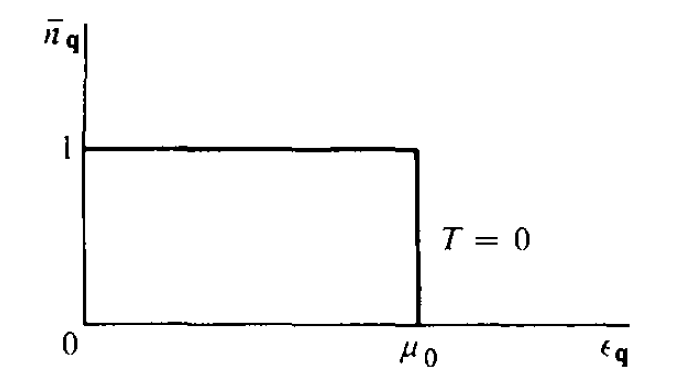
\includegraphics[width=0.5\textwidth]{Immagini/FermiStep.png}
	\vspace*{-5pt}
	\caption{}
	\label{fig:fermistep}
\end{figure}

La funzione $n_{\textbf{q}} (\varepsilon_{\textbf{q}})$ diventa quindi una funzione a gradino (vedi \cref{fig:fermistep}), in cui il punto di frontiera è $\varepsilon_{\textbf{q}} = \mu_0$, cioè il potenziale chimico a $T=0$, che è fissato dall'equazione:
\begin{equation*}
N = \lim_{T\rightarrow 0} \sum_{\textbf{q}} \frac{1}{\exp\left[(\varepsilon_{\textbf{q}} - \mu)/k_B T\right] + 1}
\end{equation*}

Anche in questo caso le somme saranno convertite in integrali, e i livelli energetici saranno considerati un insieme continuo. La giustificazione qui non può più essere data dal confronto con la scala di energia termica, che qui è nulla, ma la scala di energia rilevante qui è proprio quella indotta da $\mu_0$, ed è rispetto ad essa che i livelli energetici sono fini, ed è strettamente connesso al fatto che si sta considerando una quantità macroscopica di particelle.

Si ha dunque che l'equazione diventa\footnote{\label{note:physth} Usando il solito \textit{teorema fisico} che afferma che limiti e integrali commutano. Formalmente non funziona, ma praticamente sì. La giustificazione migliore è che le funzioni per cui fallisce hanno un comportamento particolare, concettualmente allargano infinitamente il loro supporto \textit{efficace} nel passaggio al limite, e sono una classe ristretta.}:
\begin{equation*}
N = \lim_{T\rightarrow 0} \int_{0}^{\infty} \frac{\rho(\varepsilon)}{\exp\left[(\varepsilon_{\textbf{q}} - \mu)/k_B T\right] + 1} \dd \varepsilon = \int_{0}^{\mu_0} \rho(\varepsilon) \dd \varepsilon
\end{equation*}
dove si è usato che il numero di occupazione diventa la funzione a gradino al limite.

Invece di integrare la densità di stati si può ottenere $N$ direttamente considerando che è il numero di celle unitarie di spazio delle fasi racchiuso in un volume fisico $V$ e in una sfera di raggio $p_F$ nello spazio degli impulsi, non dimenticando la degenerazione di spin. Si ottiene quindi:
\begin{equation*}
N = \frac{gV \frac{4}{3} \pi p_F^3}{(2\pi \hbar)^3}
\end{equation*}
un altro modo, forse un poco più astuto, per trovare questo risultato è sfruttare il fatto che $ \rho(\varepsilon) \propto \varepsilon^\alpha $, cioè è una funzione omogenea in $ \varepsilon $.

\noindent Dalla precedente si ottiene:
\begin{align*}
p_F &= 2\pi \hbar \left(\frac{N}{V} \frac{3}{4\pi g}\right)^{1/3}\\
\mu_0 &= \frac{p_F^2}{2m} = \frac{(2\pi \hbar)^2}{2m} \left(\frac{N}{V} \frac{3}{4\pi g}\right)^{2/3}
\end{align*}

Si nota che contrariamente al caso del gas classico il potenziale chimico $\mu_0$ è qui positivo: infatti non è possibile aggiungere particelle a energia nulla, ma solo a energia $\geq \mu_0$, inoltre non c'è bisogno di fare alcuna correzione per la variazione di entropia, che è nulla prima e dopo l'inserimento.

Il potenziale chimico $\mu_0$ è noto come \textit{energia di Fermi} $\varepsilon_F$. \`E anche nota la temperatura di Fermi $T_F$, definita da $k_B T_F = \varepsilon_F$.
\newline

Poiché anche nel caso quantistico la densità di stati di singola particella in energia è proporzionale a $\varepsilon^{1/2}$ allora:
\begin{align*}
	\bar{\varepsilon} = \frac{\int_{0}^{\varepsilon_F} \varepsilon \rho(\varepsilon) \dd \varepsilon}{\int_{0}^{\varepsilon_F} \rho(\varepsilon) \dd \varepsilon} = \frac{\int_{0}^{\varepsilon_F} \varepsilon^{3/2} \dd \varepsilon}{\int_{0}^{\varepsilon_F} \varepsilon^{1/2} \dd \varepsilon} = \frac{\frac{2}{5} \varepsilon_F^{5/2}}{\frac{2}{3} \varepsilon_F^{3/2}} = \frac{3}{5} \varepsilon_F
\end{align*}
e di conseguenza l'energia totale:
\begin{equation*}
E = \frac{3}{5} N \varepsilon_F = \frac{3(2\pi \hbar)^2}{10m} \left(\frac{N}{V} \frac{3}{4\pi g}\right)^{2/3} N
\end{equation*}
poiché l'entropia è nulla allora l'energia libera è pari all'energia $E=F$, e dunque per la pressione si ha:
\begin{equation}
P = - \partfix{F}{V}{T,N} = - \partfix{E}{V}{S,N} = \frac{2}{3} \frac{E}{V}
\end{equation}
Questa pressione finita temperatura nulla è la conseguenza estrema della forza efficace repulsiva tra fermioni che si iniziava a manifestare già in prossimità del limite classico (vedi \cref{sec:fewdegas}).

Inoltre il risultato trovato conferma la previsione generale, vista nella \cref{sec:idpart}, che per un gas perfetto $ E = \frac{3}{2} PV$, che dipende solo dalla legge di dispersione e dalla definizione di pressione, mentre ciò che differisce nei due casi è proprio l'energia: per un gas ideale a $T=0$ l'energia è nulla, e quindi anche la pressione.

\paragraph{Basse temperature} Per temperature piccole, ma non nulle, ci si aspetta che il comportamento del gas sia prossimo a quello a $T=0$, quindi si studierà tale limite in modo perturbativo.

La condizione di basse temperature è che:
\begin{equation*}
T \ll T_F
\end{equation*}

Un valore tipico per $T_F$ si può ottenere considerando l'espressione per $\varepsilon_F$ e valori tipici per le varie grandezze:
\begin{itemize}
	\item per la massa delle particelle si considera quella dell'elettrone;
	\item per la degenerazione di spin si pone $g=2$, cioè spin $1/2$;
	\item per la densità, che è la densità degli elettroni di conduzione dei metalli, si considera quella del rame, conduttore comune (in ogni caso varia di meno di un ordine di grandezza fra i vari metalli);
\end{itemize}
Il valore che si ottiene per la temperatura di Fermi è $T_F = \unit{8.5\cdot10^4}{\kelvin}$, mentre il punto di fusione del rame è $\sim \unit{10^3}{\kelvin}$, per cui finché il rame è solido gli elettroni soddisfano pienamente il limite di bassa temperatura.
\newline

Ciò che accade è che alzando la temperatura da $0$ gli elettroni sul guscio esterno acquistano un energia dell'ordine di $k_B T$, ma quelli in profondità nel \textit{mare di Fermi} non possono fare altrettanto, perché tutti gli stati accessibili tramite eccitazione termica sono già occupati.

Quindi solo gli elettroni sul guscio contribuiscono alle deviazioni rispetto al comportamento a $T=0$, e sono una frazione piccola del totale, dell'ordine di $T/T_F$ (la palla che costituisce il mare di Fermi nello spazio degli impulsi è tridimensionale, quindi non ci sono comportamenti peculiari causati da sfere di dimensionalità alta).

\begin{figure}[h!]
	\centering
	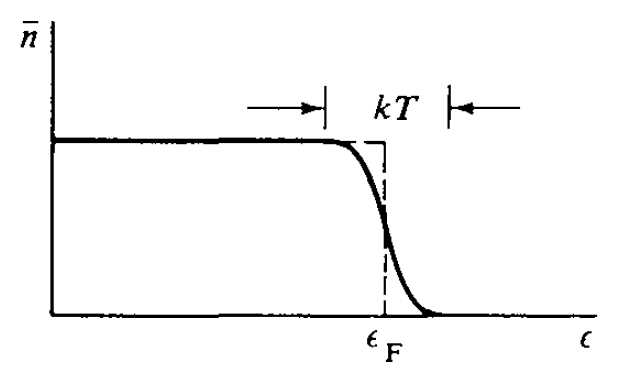
\includegraphics[width=0.5\textwidth]{Immagini/FStepT.png}
	\caption{}
	\label{fig:fstepT}
\end{figure}

La forma che assume adesso il numero medio di occupazione è simile alla precedente, ma appare più \textit{smussata} (non ci possono essere discontinuità a temperatura finita), come è mostrato in \cref{fig:fstepT}. 
Si noti che la zona interessata ha uno spessore dell'ordine di $k_B T$.
\newline

Il modello di conduzione precedente all'introduzione dei gas di Fermi era quello di Drude, esso però presentava un problema fondamentale: se gli elettroni costituivano un gas non-interagente anche loro dovevano avere una loro capacità termica, proporzionale al numero di gradi di libertà (per il teorema di equipartizione), e misurandola si è potuto fissare un limite superiore al numero di elettroni in un metallo. Il limite così trovato risultava troppo ridotto: un tale numero di elettroni non era sufficiente a dare conto delle proprietà di conduzione dei metalli.

Questo dilemma può essere risolto dal modello proposto dal gas di fermioni: tutti gli elettroni contribuiscono alla conduzione elettrica, perché l'effetto del campo è quello di spostare l'intera sfera di Fermi (la perdita di isotropia è giustificata dalla direzione individuata dal campo), mentre la conduzione termica coinvolge solo gli elettroni del guscio, cioè una frazione dell'ordine $T/T_F$ del totale, dando ragione della capacità termica ridotta rispetto al grande numero di particelle.

Ci sono però dei punti da chiarire prima di potere applicare il modello del gas di Fermi alla conduzione:
\begin{itemize}
	\item il gas che si sta considerando non è ideale, ma è pur sempre perfetto: come può esserlo un gas costituito da particelle cariche? La risposta è che gli elettroni in moto in un metallo sono immersi in una regione di carica positiva costituita dagli ioni (il metallo è globalmente neutro), per cui essi tendono a "schermarsi" con le cariche positive e costituire dei portatori efficaci, che appaiono neutri gli uni agli altri; più avanti si inserirà questo effetto nel modello;
	\item la stessa distribuzione di Fermi rende più improbabili le collisioni: gli elettroni in profondità nel mare di Fermi non possono collidere, perché il risultato della collisione sarebbe quello di raggiungere un nuovo stato, ma quelli immediatamente attorno sono occupati, e quindi le collisioni soppresse;
	\item un'ultima obiezione potrebbe essere che non si stanno considerando le collisioni con gli elementi della struttura cristallina del metallo: gli ioni positivi; il motivo per cui vengono trascurate è che gli elettroni non sono elementi localizzati nel metallo, ma gli stati di singola particella costituiti da onde, la cui lunghezza è determinata dall'impulso, ed è molto più grande della spaziatura fra gli atomi per la maggioranza degli stati coinvolti; delle onde così lunghe non possono quindi accorgersi significativamente della struttura granulare del reticolo (questo punto sarà affrontato con maggiore dettaglio nel \cref{chap:crystals}, in cui si tratterà dei cristalli).
	
	Si anticipa che legge di dispersione degli elettroni in un metallo in effetti è piuttosto diversa da quella di un gas perfetto. Quest'ultima è:
	\begin{equation*}
	\varepsilon = \frac{\hbar^2 q^2}{2 m^\ast}
	\end{equation*}
	dove con $m^\ast$ è indicata la massa efficace dei portatori dovuta alla schermatura discussa al primo punto, ed è un poco maggiore di quella degli elettroni a causa della carica positiva addizionale.
	La differenza nelle leggi di dispersione è illustrata in \cref{fig:elecdisp}.
\end{itemize}

\begin{figure}[t]
\centering
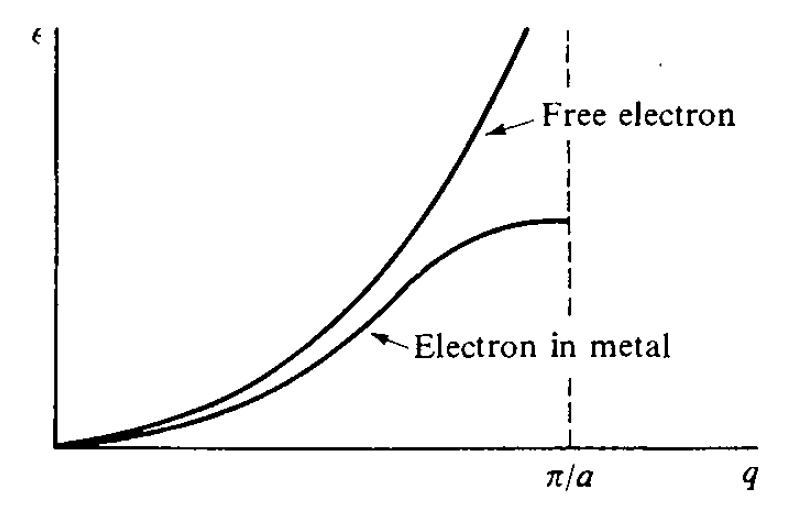
\includegraphics[width=0.5\textwidth]{Immagini/ElectronsDispersion.png}
\caption{}
\label{fig:elecdisp}
\end{figure}

Si studiano ora le proprietà termiche del gas perfetto di Fermi, partendo dalla funzione di granpartizione:
\begin{equation*}
\Omega = - k_B T \sum_{\textbf{q}} \log \left[1 + \exp \left(-\frac{\varepsilon_{\textbf{q}} - \mu}{k_B T}\right)\right] = - \kt \int_{0}^{\infty} \rho(\varepsilon)\log \left[1 + \exp \left(\frac{\mu - \varepsilon}{k_B T}\right)\right] \dd \varepsilon
\end{equation*}
Che può essere integrata per parti, oppure si può prendere una scorciatoia e considerare che (finché $\varepsilon \propto p^2$) $E = -\frac{3}{2} \Omega$, e quindi:
\begin{equation*}
\Omega =  -\frac{2}{3} E = -\frac{2}{3} \int_{0}^{\infty} \varepsilon \rho(\varepsilon)\bar{n}(\varepsilon)\dd \varepsilon = - \frac{2}{3} \frac{4\pi V g \sqrt{2} m^{3/2}}{\hplanck^3} \int_{0}^{\infty}\frac{\varepsilon^{3/2} \dd \varepsilon}{e^{(\varepsilon - \mu)/k_BT} +1}
\end{equation*}
Per valutare questa espressione si deve quindi eseguire l'integrale di una funzione che è molto vicina al gradino.
Si può quindi trattare il problema perturbativamente e trovare quale sia la correzione $\delta I$ al valore dell'integrale $I_0$ a temperatura nulla:
\begin{align*}
I = I_0 + \delta I \qquad I_0 &= \int_{0}^{\mu} f(\varepsilon) \dd \varepsilon\\
I= \int_{0}^{\infty} f(\varepsilon) \bar{n}(\varepsilon) \dd \varepsilon &= \int_{0}^{\infty}  \frac{f(\varepsilon)}{e^{(\varepsilon - \mu)/k_BT} +1} \dd \varepsilon
\end{align*}
\`E importante ricordare che la variazione in $T$ è fatta a $\mu$ costante, quindi $N$ può cambiare (se si impone il contrario il valore di $I_0$ dipenderà dalla temperatura, ma si può fare).

Sviluppando quindi $I$ in $T=0$ si ha:
\begin{equation*}
I = I_0 + \partfix{I}{T}{T=0} T + \frac{1}{2} \partfix{^2 I}{T^2}{T=0} T^2 + ~\cdots
\end{equation*}

La questione fondamentale qui è a quale ordine si trova il primo termine non nullo (dopo quello all'ordine zero ovviamente), poiché il comportamento termico sarà dominato da esso. Il risultato è che tale termine è quello al second'ordine, mentre il primo si annulla.

Il motivo per cui il termine al prim'ordine è nullo è sostanzialmente che le particelle in più con $\varepsilon_{\textbf{q}} > \mu$, appena sopra tale limite, danno un contributo a $\Omega$ quasi uguale a quello dato dalle particelle con $\varepsilon_{\textbf{q}}$ appena inferiore a $\mu$, che vengono a mancare rispetto al caso del gradino. La situazione è illustrata in \cref{fig:stepsmooth}.

\begin{figure}[b]
	\centering
	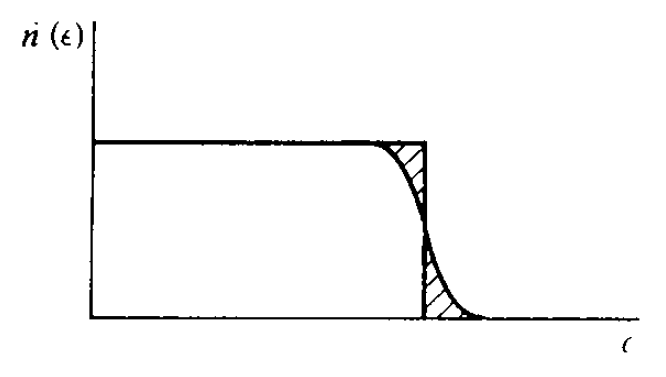
\includegraphics[width=0.5\textwidth]{Immagini/SmoothStep.png}
	\caption{}
	\label{fig:stepsmooth}
\end{figure}

Più in dettaglio si ha che il numero di particelle a una certa energia $\varepsilon$ è dato da $\rho(\varepsilon)\bar{n}(\varepsilon)$, e poiché nella zona attorno a $\mu$ la densità degli stati $\rho(\varepsilon)$ varia relativamente poco l'area tratteggiata in \cref{fig:stepsmooth} corrisponde quasi al numero di particelle che vengono promosse, e quindi il fatto che le due aree si compensino riflette il fatto che il numero di particelle è quasi conservato.
\newline

Si passa quindi alla valutazione quantitativa. Sia:
\begin{equation*}
	z = \frac{\varepsilon - \mu}{k_B T}
\end{equation*}

Si possono definire due funzioni di $z$, $g_0(z)$ e $g_1(z)$, che rappresentino le aree tratteggiate, cioè la differenza tra il gradino e il numero medio di occupazione a temperatura finita, e che quindi siano significativamente diverse da $0$ solo in un intorno di $z=0$, come mostrato in \cref{fig:stepdiffunc}.

\begin{figure}[t]
	\centering
	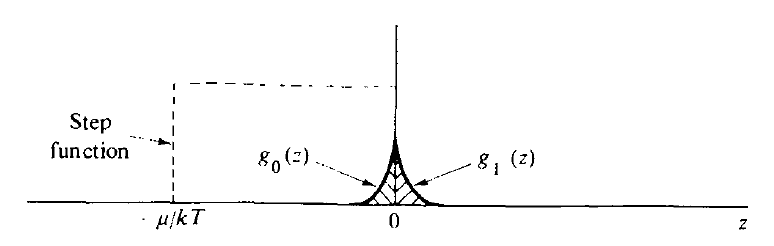
\includegraphics[width=0.7\textwidth]{Immagini/SmoothStepDifferences.png}
	\caption{}
	\label{fig:stepdiffunc}
\end{figure}

Si ottiene quindi:
\begin{equation*}
\delta I \approxeq \int_{-\infty}^{\infty} f(\varepsilon)[g_1(z) - g_0(z)] \dd \varepsilon = \int_{-\infty}^{\infty} f(\mu + k_B T z)[g_1(z) - g_0(z)] \kt \dd z
\end{equation*}
i limiti di integrazione considerati non introducono un ulteriore approssimazione perché al di fuori della regione di integrazione precedente il valore delle funzioni $g$ è praticamente nullo ovunque.

Si espande quindi $f$ in $z=0$ e si sostituisce in $\delta I$:
\begin{align*}
f(\mu + \kt z) &= f(\mu) + \kt z \partfix{f}{\varepsilon}{\varepsilon = \mu} + \cdots = f(\mu) + \kt z f'(\mu) + \cdots\\
\delta I &= \kt f(\mu) \int_{-\infty}^{\infty} [g_1(z) - g_0(z)] \dd z + (\kt)^2 f'(\mu) \int_{-\infty}^{\infty} z[g_1(z) - g_0(z)] \dd z
\end{align*}
il primo termine è quindi effettivamente proporzionale alla differenza di aree. Inoltre, se il primo termine si annulla sarà perché la funzione è approssimativamente dispari, e quindi si annulleranno tutti i termini di ordine dispari. D'altro canto il secondo termine non può annullarsi perché è sempre positivo.

Si esaminano quindi le funzioni $g$:
\begin{align*}
g_1(z) &= \frac{1}{e^z + 1}	\qquad (z \geq 0)\\
g_0(z) &= 1 - \frac{1}{e^z + 1} = \frac{e^z}{e^z + 1} = \frac{1}{1 + e^{-z}} \qquad (z < 0)
\end{align*}
ottenute considerando che $g_1$ coincide sostanzialmente con $\bar{n}$ e $g_0$ con $1 - \bar{n}$, per entrambi sul loro supporto.

Da queste espressioni si ottiene quindi:
\begin{align*}
	\int_{-\infty}^{\infty} [g_1(z) - g_0(z)] \dd z &= \int_{0}^{\infty} g_1(z) \dd z - \int_{-\infty}^{0} g_0(z) \dd z = \int_{0}^{\infty} \frac{\dd z}{e^z + 1} - \int_{-\infty}^{0} \frac{\dd z}{1 + e^{-z}} =\\
	&= \cdots ~+ \int_{+\infty}^{0} \frac{\dd z}{1 + e^{z}} = \cdots ~- \int_{0}^{\infty} \frac{\dd z}{1 + e^{z}} = 0
\end{align*}
mentre per il secondo termine:
\begin{equation*}
\int_{-\infty}^{\infty} z [g_1(z) - g_0(z)] \dd z = 2 \int_{0}^{\infty} \frac{z\dd z}{e^z + 1} = \frac{\pi^2}{6}
\end{equation*}

La formula per l'espansione di $I$ al quart'ordine\footnote{Qui abbiamo motivato, ed è sufficiente, il secondo} è:
\begin{equation*}
I = \int_{0}^{\mu} f(\varepsilon) \dd \varepsilon +  \frac{\pi^2}{6} f'(\mu) (\kt)^2 + \frac{7\pi^4}{360} f'''(\mu) (\kt)^4 + \cdots
\end{equation*}
e infine per la funzione di granpartizione:
\begin{equation*}
\Omega = - \frac{2}{3} \frac{4\pi V g \sqrt{2} m^{3/2}}{\hplanck^3}\left[\frac{2}{5}\mu^{5/2} + \frac{\pi^2}{4} \mu^{1/2} (\kt)^2\right]
\end{equation*}

Da quest'ultima è possibile ricavare il numero di particelle:
\begin{equation*}
N = - \partfix{\Omega}{\mu}{V,T} = - \frac{2}{3} \frac{4\pi V g \sqrt{2} m^{3/2}}{\hplanck^3}\left[\mu^{3/2} + \frac{\pi^2}{8} \frac{(\kt)^2}{\mu^{1/2}}\right]
\end{equation*}
e dall'espressione del numero di particelle a temperatura nulla $N_0$ si ha che:
\begin{align*}
N_0 &= \frac{2}{3} \frac{4\pi V g \sqrt{2} m^{3/2} \mu^{3/2}}{\hplanck^3}\\
N &= N_0\left[1 + \frac{\pi^2}{8} \left(\frac{\kt}{\mu}\right)^2\right]
\end{align*}

Questo è il risultato trovato considerando il caso grancanonico, in cui $\mu$ è fisso e il numero totale di particelle $N$ può cambiare attingendo alla riserva,
Si può invece considerare $N$ fisso e $\mu$ variabile, che è una situazione che si presenta frequentemente, specialmente in ambito sperimentale (ma non necessariamente, il campione ad esempio potrebbe essere parte di un circuito elettrico).

Il numero delle particelle sarà quindi:
\begin{equation*}
N = N_0\left[1 + \frac{\pi^2}{8} \left(\frac{\kt}{\mu}\right)^2\right]\left(\frac{\mu}{\mu_0}\right)^{3/2}
\end{equation*}
poiché $N_0 \propto \mu^{3/2}$, in modo da riprodurre il risultato precedente. Imponendo quindi $N = N_0$ si trova $\mu_0$:
\begin{equation*}
\mu \simeq \frac{\mu_0}{\left[1 + {\pi^2}/{8} \left({\kt}/{\mu_0}\right)^2\right]^{2/3}} \simeq \mu_0 \left[1 - \frac{\pi^2}{12} \left(\frac{\kt}{\mu_0}\right)^2\right]
\end{equation*} 
in cui nella prima uguaglianza si è posto $\mu = \mu_0$ nel membro di destra, per limitarsi all'approssimazione al primo ordine non nullo, mentre nella seconda uguaglianza si sviluppato il denominatore.

Era prevedibile, ma non ovvio: ad alte temperature si recupera il limite classico, per cui $\mu$ deve diventare negativo e grande con l'alzarsi della temperatura.
\newline

A partire dalla funzione di granpartizione si può anche ricavare l'entropia:
\begin{equation*}
S = - \partfix{\Omega}{T}{V, \mu} = \frac{4\pi V g \sqrt{2} m^{3/2}}{\hplanck^3} \frac{\pi^2}{3} \mu^{1/2} k_B^2 T 
\end{equation*}
che è la funzione $S(T,V,\mu)$, piuttosto che $S(T,V,N)$; ma si sa che una variazione di $ \mu $ con $  N $ costante è dell'ordine $ T^3 $, quindi trascurabile rispetto alle altre.

Si può quindi scrivere:
\begin{equation*}
S = \frac{\pi^2}{2} N k_B \frac{T}{T_F}
\end{equation*}
e quindi ottenere la capacità termica a volume costante:
\begin{equation*}
C_V = T \partfix{S}{T}{V} = \frac{\pi^2}{2} N k_B \frac{T}{T_F}
\end{equation*}
in accordo a quanto affermato precedentemente sul fatto che per i fenomeni termici sono rilevanti solo gli elettroni del guscio, con una frazione tipica data da $T/T_F$

Si trova che il risultato sperimentale è in accordo con l'andamento lineare, ma differisce nelle costanti, infatti:
\begin{align*}
\frac{C_V}{N \kt} &= 0.8 \cross 10^{-4} \qquad (\text{experimental})\\
\frac{C_V}{N \kt} &= 0.6 \cross 10^{-4} \qquad (\text{predicted})
\end{align*}

Questa differenza può essere colmata in base alla considerazione fatta all'inizio della sezione sulla massa efficace dovuta alla schermatura, infatti $C_V \propto T_F^{-1} \propto m$ per cui una massa $m^\ast \simeq 1.3 m$ da ragione del valore leggermente più alto ottenuto sperimentalmente.
\newline

Nella discussione fatta ci sono alcuni punti che sono stati trascurati:
\begin{itemize}
	\item i cristalli non sono isotropi, per cui il mare di Fermi anziché avere la forma di una sfera nello spazio degli impulsi a forme più complesse, e l'impulso di Fermi può dipendere in generale dalla direzione lungo cui lo si valuta;
	\item gli elettroni non interagiscono con gli atomi del cristallo nelle loro posizioni di equilibrio, ma possono interagire con le impurità del cristallo e con il moto di eccitazine termica del reticolo (i fononi).
\end{itemize}
Inoltre potrebbe essere naturale essere scettici riguardo al ruolo della massa efficace, in particolare essa appare come un parametro libero che viene fissato ad hoc per rendere la teoria in accordo con la realtà sperimentale.
Si è però provato che non è esattamente così: studiando il moto degli elettroni in un cristallo sotto l'azione di un campo magnetico si è riusciti a determinare che gli elettroni si comportano, per distanze dell'ordine del libero cammino medio, come particelle cariche in un ciclotrone, con una frequenza:
\begin{equation*}
\omega_c = \frac{e H}{m^\ast c}
\end{equation*}
in questo modo si è misurato in modo indipendente il valore di $m^\ast$.

Il valore trovato in questo modo dipende dalla direzione, a causa proprio dell'anisotropia dei cristalli, ma una volta opportunamente mediato esso è in ottimo accordo con i dati ottenuti dallo studio delle capacità termiche.

\section{Gas di Bose molto degenere: condensati di Bose-Einstein}
\label{sec:bosegas}

Le equazioni trovate nella \cref{sec:BFstat} per il gas di Bose sono estremamente simili in forma a quelle relative al gas di Fermi. I risultati a cui conducono sono però completamenti differenti.
\newline

Si inizia studiando il numero di particelle in un gas di Bose, dato da:
\begin{equation*}
N = \sum_{\textbf{q}}  \frac{1}{ \exp\left[(\varepsilon_{\textbf{q}} - \mu)/k_B T\right] - 1}
\end{equation*}
e considerando che a temperatura finita la spaziatura tra i livelli è piccola in confronto all'energia termica (le grandezze che vanno confrontate sono la lunghezza d'onda termica con le dimensioni lineari del sistema) si può immediatamente convertire in un integrale:
\begin{equation*}
N =  \frac{4\pi V g \sqrt{2} m^{3/2}}{\hplanck^3} \int_{0}^{\infty}  \frac{\varepsilon^{1/2} \dd \varepsilon}{ \exp\left[(\varepsilon - \mu)/k_B T\right] - 1}
\end{equation*}

Inoltre nel caso del gas di Bose il potenziale chimico è strettamente negativo (al contrario nel caso dei fermioni era positivo).

Si consideri ora la situazione di un gas in un contenitore a  $V$ fissato e in contatto con un bagno termico, che quindi fissa $ T $. Si consideri che il sistema non si ain grado di scambiare particelle con una riserva, e quindi $N$ è fissato, ma con la possibilità di aggiungere particelle dall'esterno (trovando nuovi stati di equilibrio di volta in volta).

L'unica variabile libera nell'equazione scritta per $ N $ è $ \mu $, e $ N(\mu) $ è una funzione crescente. Poiché $\mu$ deve rimanere negativo è lecito chiedersi se esitìstono valori finiti di $ N $ per cui il potenziale chimico raggiunge il suo limite. Si impone quindi $ \mu = 0$ e si calcola il numero totale di particelle:
\begin{align*}
N &=  \frac{4\pi V g \sqrt{2} m^{3/2}}{\hplanck^3} (\kt)^{3/2} \int_{0}^{\infty}  \frac{x^{1/2} \dd x}{ e^x - 1}\\
&\int_{0}^{\infty}  \frac{x^{1/2} \dd x}{ e^x - 1} \simeq 2.31 \simeq \frac{\sqrt{\pi}}{2} \cdot 2.612
\end{align*}
ottenendo quindi una densità critica di particelle, o una temperatura critica (se si immagini di abbassare la temperatura a densità costante):
\begin{align*}
\left(\frac{N}{V}\right)_c &= \frac{2.612}{\Lambda^3}\\
T_c &= \frac{1}{2.31 m k_B} \left(\frac{N}{V}\right)^{2/3} \frac{(\hplanck)^2}{(4\pi \sqrt{2})^{2/3}}
\end{align*}
La presenza di una densità critica, espressa direttamente come funzione di $\Lambda$, rende conto del fatto che le particelle non possono più essere localizzate senza sovrapporsi quantisticamente.
\newline

Il problema è quindi il seguente: non ci sono ragioni evidenti per cui il sistema non possa contenere ulteriori particelle oltre le densità critica, a $ T $ e $ V $ fissati, ma poiché il potenziale chimico non può più crescere il conteggio rimane fisso al valore trovato per $ \mu = 0 $.

La soluzione può essere compresa per analogia con un problema noto: in un gas ideale (ad esempio azoto N$_2$, a una temperatura di $ ~\unit{60}{\kelvin} $, appena sopra al punto triplo) $N = (V/\kt) P$, per cui a $ V $ e $ T $ fissati la pressione dovrebbe essere direttamente proporzionale al numero di particelle, ma sperimentalmente anche aumentando $ N $ a un certo punto la pressione si assesta su un valore costante: il gas sta subendo una transizione di fase, e la curva si assesta sulla pressione di vapore e le nuove particelle sono bilanciate da quelle che passano alla fase liquida. In \cref{fig:gastoliquid} si riporta il comportamento descritto.

\begin{figure}[t]
	\centering
	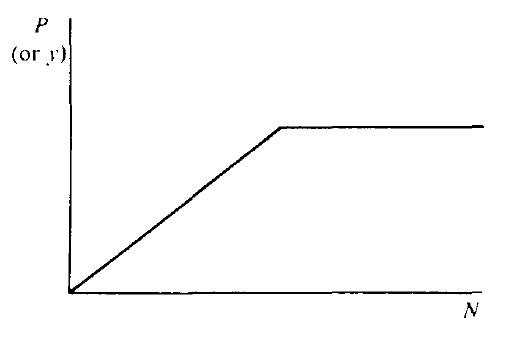
\includegraphics[width=0.5\textwidth]{Immagini/GasToLiquid.png}
	\vspace{-10pt}
	\caption{}
	\label{fig:gastoliquid}
	\vspace{-10pt}
\end{figure}

Si ottiene una figura analoga se si riporta su un grafico il caso del gas di Bose, mantenendo in ascissa $ N $ e ponendo in ordinata:
\begin{equation*}
	y =  \int_{0}^{\infty}  \frac{\varepsilon^{1/2} \dd \varepsilon}{ \exp\left[(\varepsilon - \mu)/k_B T\right] - 1}
\end{equation*}

La domanda diventa quindi: perché il conteggio delle particelle sta perdendo traccia di alcune di esse? Si riesamina quindi il procedimento adoprato.
\begin{itemize}
	\item Potrebbe essere a causa dell'approssimazione fatta integrando sugli stati, anziché sommare; essa è giustificata se il sistema soddisfa:
	\begin{equation*}
		\kt \gg \frac{\hbar^2}{2m} \left(\frac{2\pi}{L}\right)^2
	\end{equation*}
	Si sostituisce quindi la temperatura critica $ T_c $, e poiché $L^2 = V^{2/3}$ il risultato dipende solo dal numero di particelle:
	\begin{equation*}
	N^{2/3} \gg \frac{2.31(4\pi\sqrt{2})^{2/3}}{2}
	\end{equation*}
	ma il secondo membro è una costante dell'ordine dell'unità, perciò per qualunque numero macroscopico di particelle l'approssimazione è ben verificata.
	
	\item Potrebbe essere dovuto della densità di stati (e lo è); nel ricavare la densità di stati si è considerata una particella libera nel vuoto, ma questa è solo un'approssimazione se il volume in cui è confinata è finito.
	
	Gli stati quindi non sono realmente stati del continuo, ma discreti, per cui la densità di stati dovrebbe prevedere la presenza di uno stato anche a energia nulla \footnote{quasi in realtà, ma tende a $0$ con le dimensioni del sistema}, cioè il fondamentale. 
	
	Questo non ha creato problemi nel gas ideale e in quello di Fermi: nel primo il numero di occupazione di ogni stato è piccolo per ipotesi, e nel secondo è $\leq g$ (la degenerazione di spin), per cui trascurare uno stato non può portare a effetti statisticamente rilevanti.
	
	Per il gas di Bose invece:
	\begin{equation*}
		\overline{n_0} = \frac{1}{e^{-\mu/\kt} - 1} \qquad \implies \qquad \overline{n_0} \simeq - \frac{\kt}{\mu} \qquad (\mu \rightarrow 0)
	\end{equation*}
	perciò quando il potenziale chimico si annulla il numero di particelle nel fondamentale diventa macroscopico, e si può identificare proprio con il fondamentale la nuova fase in equilibrio con il gas di Bose, ritrovando le particelle mancanti nel conteggio.
	
	Tale fase è detta \textit{condensato di Bose-Einstein}.
\end{itemize}

\subsubsection{Proprietà del condensato di Bose-Einstein}

Le particelle che non sono nel fondamentale sono tutte correttamente incluse nel conteggio fatto per $ N $. Chiameremo ora questo numero $ N^\star $, per distinguerlo dal numero complessivo di particelle del sistema, che sarà sempre $ N $.
Si ha quindi:
\begin{equation*}
N^\star = \int_{0}^{\infty}  \frac{\rho(\varepsilon) \dd \varepsilon}{ e^{\varepsilon/k_B T} - 1} = N \left(\frac{T}{T_C}\right)^{3/2} \qquad \qquad \text{per } T < T_c
\end{equation*}
mentre per le particelle nel fondamentale si ha:
\begin{equation*}
	N_0 = N - N^\star = N \left[1 - \left(\frac{T}{T_C}\right)^{3/2}\right] \qquad \qquad \text{per } T > T_c
\end{equation*}

L'energia del gas è tutta nelle particelle $ N^\star $, essendo le altre nel fondamentale, e quindi a energia nulla.
\begin{equation*}
	E = \int_{0}^{\infty}  \frac{\varepsilon \rho(\varepsilon) \dd \varepsilon}{ e^{\varepsilon/k_B T} - 1} = \frac{4\pi V g \sqrt{2} }{\hplanck^3} (m\kt)^{3/2} \kt \int_{0}^{\infty}  \frac{x^{3/2} \dd x}{ e^x - 1}
\end{equation*}

\begin{note}[Integrali notevoli]
	Tutti gli integrali nella forma in cui è posto quello nell'espressione precedente possono essere valutati per mezzo di \textit{funzioni speciali}:
	\begin{equation*}
		\int_{0}^{\infty}  \frac{x^n \dd x}{ e^x - 1} = \Gamma(n+1) \zeta(n+1)
	\end{equation*}
	dove $ \Gamma(\cdot) $ è la funzione \textit{gamma di Eulero} e $ \zeta(\cdot) $ è la funzione \textit{zeta di Riemann}.
\end{note}

Nel caso in esame si ha:
\begin{equation*}
	\int_{0}^{\infty}  \frac{x^{3/2} \dd x}{ e^x - 1} = \frac{3\sqrt{\pi}}{4} \cdot 1.341
\end{equation*}
per cui l'energia è:
\begin{equation*}
	E = 0.770 \kt N^{\star} = 0.770 \kt N  \left(\frac{T}{T_C}\right)^{3/2}
\end{equation*}
perciò la dipendenza dalla temperatura dell'energia è $ E \propto T^{5/2} $. Conseguentemente la capacità termica è:
\begin{equation*}
	C_V = \partfix{E}{T}{V,N} = 1.9 k_B N  \left(\frac{T}{T_C}\right)^{3/2} = 1.9 N^\star k_B 
\end{equation*}
e quindi dal punto di vista della capacità termica il comportamento della parte eccitata non è molto diverso da quello del gas ideale, in cui $C_V = 1.5 N k_B$.

\begin{figure}[t]
	\centering
	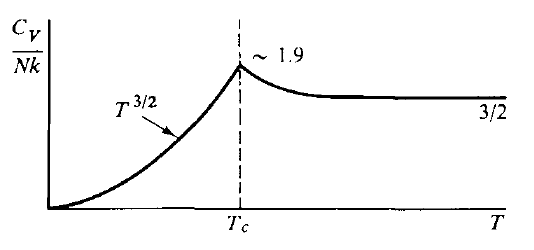
\includegraphics[width=0.6\textwidth]{Immagini/BoseThermalCapacity.png}
	\vspace{-10pt}
	\caption{}
	\label{fig:thermcapbose}
	\vspace{-10pt}
\end{figure}

Si riporta il grafico della capacità termica in funzione della temperatura, in esso sono chiari i seguenti andamenti:
\begin{itemize}
	\item per temperature inferiori alla temperatura critica la capacità termica per singola particella va come $ T^{3/2} $, cioè è proporzionale alla frazione di particelle non condensate;
	\item per temperature molto maggiori della temperatura critica la capacità termica per singola particella tende ad assestarsi su un valore costante, cioè $ 1.5 k_B $, il valore del gas ideale;
	\item per temperature maggiori alla temperatura critica, avvicinandosi ad essa, il comportamento del gas si fa meno ideale, e inizia ad agire la forza efficace tra bosoni, per cui la capacità termica sale leggermente oltre il suo valore ideale a causa di tali interazioni efficaci, fino al valore di $ 1.9 k_Bf $.
\end{itemize}

\subsection{Tecniche di realizzazione sperimentale di un condensato di Bose-Einstein}

% TODO: qui devo chiedere a Albe o Hoch che erano presenti di scriverla al posto mio

\subsection{Approfondimenti sui condensati}
Ci sono due ulteriori argomenti elementari d'interesse legati alla condensazione di Bose:
\begin{itemize}
	\item lo studio e la classificazione della transizione di fase;
	\item la condensazione nello spazio fisico.
\end{itemize}

Il primo punto è connesso ad alcuni aspetti della teoria generale sulle transizioni di fase, cioè l'ordine della transizione: la condensazione è effettivamente una transizione del primo ordine, con un calore latente associato, anche se da quanto discusso non appare (la capacità termica è continua, e quindi a maggior ragione lo è l'entropia, ma si è studiato tutto a volume costante, mentre per caratterizzare adeguatamente la transizione di fase è necessario imporre che sia la pressione ad essere costante).
\newline

Il secondo punto riguarda il tipo di condensazione: il fondamentale è un autostato dell'impulso, quindi infinitamente delocalizzato sul volume disponibile. Eppure risulta che a pressione $ P $ e temperatura $ T $ costanti si può portare il \textit{vapore di Bose} (la porta non condensata in coesistenza) a passare tutto nella fase condensata mediante compressione, e il processo termina quando tutte le particelle del vapore finiscono nel condensato, e questo avviene a $ V = 0 $.

Per questo si può affermare che la condensazione avvenga anche nello spazio fisico.

% TODO: Potrei scrivere un appendice con gli argomenti tralasciati sulla condensazione.

\begin{note}[Letture consigliate]
	Per approfondire questi due argomenti si consiglia di leggere il \textit{Goodstein}, in particolare le pagine dalla $ 132 $ alla $ 139 $.
\end{note}

\section{Elettroni}

Si raccolgono in questa sezione diversi argomenti che riguardano in particolare l'applicazione dei concetti statistici esposti nel \cref{chap:termstat} e quelli riguardanti i fermioni in questo.

\subsection{Conduzione nei metalli}
\label{sec:elecconduct}

Il trasporto di corrente elettrica da parte degli elettroni in un metallo, sotto l'azione di un campo esterno, è dovuto all'azione simultanea dell'accelerazione prodotta dal campo e dalla perdità di energia e quantità di moto nelle collisioni con le impurità.

\subsubsection{Modello di Drude}
Sotto l'azione del campo esterno $ E $ gli elettroni subiscono un'accelerazione $ a = e E /m $ in direzione opposta al campo, con $ e $ e $ m $ rispettivamente la carica e la massa dell'elettrone.

In assenza di campo gli elettroni si muovono termicamente, per cui la media della distribuzione delle velocità è nulla $ \expval{v_0} = 0 $. Si ha quindi che in presenza di campo:
\begin{align*}
\expval{\Delta v} = \expval{v} \qquad \text{con}~ \Delta v = v - v_0
\end{align*}
si ha quindi per la corrente:
\begin{equation*}
J = n e \expval{v} = n e \expval{\Delta v}
\end{equation*}
con $ n $ la densità di elettroni.

Introducendo un termine di attrito\footnote{Esso condurrà a un'evoluzione esponenziale verso l'equilibrio, che si può giustificare sulla base della teoria delle perturbazioni dipendenti dal tempo.} si ottiene l'equazione:
\begin{equation*}
\derivative{\expval{\Delta v}}{t} = e \frac{E}{m} - \frac{\expval{\Delta v}}{\tau_c}
\end{equation*}
dove si è introdotto un tempo caratteristico $ \tau_c $. L'equazione precedente ha uno stato stazionario:
\begin{equation*}
\expval{\Delta v} = \frac{e \tau_c}{m} E
\end{equation*}
per cui la corrente e la conducibilità risultanti sono:
\begin{equation*}
J = e^2 n \frac{E \tau_c}{m} \qquad \implies \qquad \sigma = \frac{J}{E} = \frac{n e^2 \tau_c}{m}
\end{equation*}

\subsubsection{Modello di Drude quantistico}

Il modo corretto di tenere conto della distribuzione di Fermi-Dirac è quello esposto nella sezione seguente, basato sull'equazione del trasporto di Boltzmann. Si può però ottenere un risultato quantitativamente corretto a partire da delle considerazioni sul gas di Fermi, che in parte sono già state esaminate nella \cref{sec:fermigas}.

Gli elettroni che contribuiscono alla conduzione sono solo quelli del guscio esterno del mare di Fermi, la cui velocità è data da:
\begin{equation*}
\frac{1}{2} m v^2 = \mu \qqimplies v = \sqrt{\frac{2\mu}{m}}
\end{equation*}
dove $ \mu $ è il potenziale chimico.

Il numero di elettroni che contribuiscono è dato dalla densità di stati in energia:
\begin{equation*}
\frac{\rho(\varepsilon) \Delta \varepsilon}{V} = \frac{3 n}{2 \mu^{3/2}} \sqrt{\varepsilon} \Delta \varepsilon
\end{equation*}
con $ \varepsilon $ l'energia degli elettroni di conduzione, e quindi $ \varepsilon = \mu $. L'intervallo di energia degli elettroni coinvolti è invece determinato dall'energia messa a disposizione dal campo per il singolo elettrone:
\begin{equation*}
\Delta \varepsilon = e E l = e E v \tau_c
\end{equation*}
dove $ l $ è il \textit{libero cammino medio}, cioè si sta considerando come energia disponibile la differenza di potenziale che può accelerare un elettrone senza che esso collida. 

Si ottiene quindi per corrente e conducibilità:
\begin{align*}
J &= e \rho(\mu) v \Delta \varepsilon = e \frac{3n}{2 \mu^{3/2}} \sqrt{\mu} e E v^2 \tau_c = \frac{3ne^2 \tau_c}{m} E\\
\sigma &= \frac{3ne^2 \tau_c}{m}
\end{align*}

Il risultato ottenuto è qualitativamente equivalente a quello del modello classico, ciò che differisce sostanzialmente è l'interpretazione. Nel caso classico tutti gli elettroni contribuiscono alla conduzione, da cui il fattore $ n $ nella conducibilità. Nel caso quantistico solo gli elettroni del guscio conducono, ma il fattore $ n $ compare lo stesso: esso è dovuto all'energia dei fermioni del guscio, cioè a quanto è profondo il mare di Fermi, e quindi è determinata da $ n $.

\subsubsection{Equazione del trasporto di Boltzmann}

Si analizza ora il fenomeno della conduzione esaminando l'evoluzione della distribuzione nello spazio delle fasi.
\newline

Si considera come spazio delle fasi di singola particella $ \dd^3 r \dd^3 v $, in cui si è scritta la velocità delle particelle anziché gli impulsi, ma in assenza di campo magnetico (o in generale di interazioni che coinvolgano la velocità delle particelle, oltre alle posizioni) questo è del tutto equivalente; infatti impulsi e velocità sono proporzionali attraverso la massa delle particelle, che qui è pure la stessa per tutti i componenti del sistema.

Sia quindi $ f(t,\textbf{r},\textbf{v}) $ il numero di particelle contenute del volumetto di spazio delle fasi di singola particella al tempo $ t $ (cioè la densità di probabilità nello spazio delle fasi di singola particella).
\footnote{Per l'esattezza si indica la densità di probabilità di occupazione con $ f(t,\textbf{r},\textbf{v})  $, mentre il numero delle particelle sarà $ f g \dd^3 r \dd^3 v $, dove $ g $ è il numero complessivo di celle dello spazio delle fasi a disposizione delle particelle.}

Dal teorema di Liouville si ha:
\begin{equation*}
f(t + \dd t,\textbf{r} + \dd \textbf{r},\textbf{v} + \dd \textbf{v}) = f(t,\textbf{r},\textbf{v}) 
\end{equation*}
per descrivere i processi dissipativi si deve però includere un termine di perdita nell'evoluzione da $ t $ a $ t + \dd t $, esso sarà dovuto alle collisioni. L'equazione diventa quindi:
\begin{equation*}
f(t + \dd t,\textbf{r} + \dd \textbf{r},\textbf{v} + \dd \textbf{v}) - f(t,\textbf{r},\textbf{v}) = \dd t \partfix{f}{t}{\text{coll}}
\end{equation*}
e si ottiene, dividendo per $ \dd t $:
\begin{equation*}
\partdev{f}{t} + \textbf{v} \grad_r f + \textbf{a} \grad_v f = \partfix{f}{t}{\text{coll}}
\end{equation*}
quest'ultima è detta \textit{equazione del trasporto di Boltzmann}.

L'ipotesi più semplice per le collisioni è supporre un andamento smorzato:
\begin{equation*}
\partfix{f}{t}{\text{coll}} = - \frac{f - f_0}{\tau_c}
\end{equation*}
$ f_0 $ rappresenta la distribuzione delle particelle nello spazio delle fasi all'equilibrio.

\begin{es}[Sistema isolato]
	Nel caso in cui i gradienti nell'equazione del trasporto di Boltzmann, prodotti dagli agenti esterni\footnote{Citazione dall'\textit{Arimondo}, pag.88; questa frase mi sembra inutile e falsa.}, siano nulli, e quindi $ f $ sia uniforme, l'equazione diventa:
	\begin{equation*}
	\partdev{f}{t} = -  \frac{f - f_0}{\tau_c}
	\end{equation*}
	e la soluzione è:
	\begin{equation*}
	(f-f_0)(t) = -  (f - f_0)e^{-\frac{t}{\tau_c}}
	\end{equation*}
	cioè evolve esponenzialmente verso lo stato di equilibrio (anche quest'ultimo dovrà essere a gradienti nulli, altrimenti essi contribuiranno nell'equazione subito dopo l'istante iniziale).
\end{es}

Il termine $ \tau_c $, che descrive il tempo caratteristico introdotto dalle collisioni, può essere modificato dall'azione di campi esterni. Tuttavia la forma del termine collisionale è giustificato dalla teoria delle perturbazioni dipendenti dal tempo, quindi, in linea con l'approccio perturbativo, si trascurerà la possibile dipendenza di $ \tau_c $ dagli agenti esterni.

\paragraph{Trasporto di carica} Si applica un campo elettrico esterno $ E $, e si cerca lo stato stazionario $ \partial f / \partial t = 0 $, che però non rappresenta lo stato di equilibrio termodinamico, che è sempre $ f_0 $.

Per lo stato stazionario l'equazione di Boltzmann sarà:
\begin{equation*}
\textbf{v} \grad_r f + \textbf{a} \grad_v f =  -  \frac{f - f_0}{\tau_c}
\end{equation*}
Si supponga inoltre che il campo elettrico sia diretto lungo l'asse $ \textbf{x} $, perciò nell'equazione il contributo delle altre direzioni sarà nullo.

Si ottiene quindi:
\begin{equation*}
f = f_0 - \tau_c(\textbf{v} \grad_r f + \textbf{a} \grad_v f) \simeq f_0 - \tau_c(\textbf{v} \grad_r f_0 + \textbf{a} \grad_v f_0)
\end{equation*}
dove si è approsimato $ f $ con $ f_0 $ nel secondo membro, in accordo con il calcolo dell'ordine perturbativo più basso.

Per elettroni nella distribuzione di Fermi-Dirac:
\begin{equation*}
f_0 (\varepsilon) = \frac{1}{\exp(\frac{\varepsilon - \mu}{\kt}) + 1}
\end{equation*}
da cui:
\begin{align*}
\partdev{f_0}{x} &= \partdev{f_0}{\mu} \partdev{\mu}{x} + \partdev{f_0}{T} \partdev{T}{x}\\
\partdev{f_0}{v_x} &= \partdev{f_0}{\varepsilon} \partdev{\varepsilon}{v_x} = m v_x \partdev{f_0}{\varepsilon}
\end{align*}
nel caso della conduzione elettrica si porrà però nullo il gradiente di temperatura $ \partial T / \partial x = 0 $, e ci si limita a esaminare il comportamento di un elemento di volume dentro il quale $ \partial N / \partial x = 0 $ (da cui si deduce $ \partial \mu / \partial x = 0$).

Imponendo infine che l'accelerazione sia $ a = e E / m $, cioè quella determinata dal campo elettrico, si ottiene:
\begin{equation*}
f \simeq f_0 - \tau_c \frac{e E}{m} m v_x \partdev{f_0}{\varepsilon}
\end{equation*}
All'ordine più basso, per il caso realistico di temperature basse rispetto a quella di Fermi (vedi \cref{sec:fermigas}), si ha:
\begin{equation*}
\partdev{f_0}{\varepsilon} = - \delta (\varepsilon - \mu_0)
\end{equation*}
dove è stato posto $ \mu = \mu_0  $, cioè il potenziale chimico a temperatura nulla, coerentemente con l'approssimazione fissata.
Inoltre per la conduzione elettrica la densità di corrente nella direzione dell'asse $ x $ è definita come:
\begin{equation*}
J_x = \int f(\textbf{x},\textbf{v})~ e v_x \rho(\textbf{v}) \dd^3 v
\end{equation*}
dove $ \rho(\textbf{v}) $ è la densità di stati nelle velocità, calcolata in assenza di campo elettrico (infatti il contributo dato dagli agenti esterni opera sull'occupazione degli stati $ f $, e non sulla densità $ \rho $).

Si ottiene quindi:
\begin{equation*}
J_x = \int e v_x f_0 \rho(\textbf{v}) \dd^3 v - e^2 E \int \tau_c v_x ^2 \partdev{f_0}{\varepsilon} \rho(\textbf{v}) \dd^3 v
\end{equation*}
in cui il primo integrale si annulla poiché l'integrando è dispari in $ v_x $ (non dipendendo dai campi esterni la funzione $ \rho(\textbf{v}) $ non può che essere pari), mentre il secondo termine è:
\begin{equation*}
J_x = e^2 E \int \tau_c  v_x ^2 \delta (\varepsilon - \mu_0) \rho(\textbf{v}) \dd^3 v
\end{equation*}

Utilizzando coordinate polari si ha:
\begin{align*}
v_x &= v \cos \theta\\
v_x^2 &= v^2 \cos^2 \theta = \frac{2 \varepsilon}{m} \cos^2 \theta\\
\rho(\textbf{v}) \dd^3 v &= \rho(\varepsilon) \dd \varepsilon \frac{\sin \theta \dd \theta \dd \varphi}{4\pi}
\end{align*}
e quindi:
\begin{align*}
J_x &= e^2 E \frac{2}{m} \int_0^\infty \tau_c \delta (\varepsilon - \mu_0) \varepsilon \rho(\varepsilon) \dd \varepsilon \frac{1}{2} \int_0^\pi \cos^2 \theta \dd \cos\theta \dd \sin\theta =\\
&= e^2 E \frac{2}{m} \frac{3n}{2 \mu_0^{3/2}} \int_0^\infty \tau_c \delta (\varepsilon - \mu_0) \frac{1}{3} \varepsilon \sqrt{\varepsilon} \dd \varepsilon = \frac{e^2 E}{m} n \tau_{c,F}
\end{align*}
dove si è indicato con $ \tau_{c,F} $ il tempo di collisione per elettroni al livello di Fermi. Si trova infine una conduttività elettrica pari a:
\begin{equation*}
\sigma = \frac{n e^2}{m} \tau_{c,F}
\end{equation*}
che è identica a quanto trovato nel caso classico, come preannunciato, ma l'interpretazione è quella data relativamente al \textit{modello di Drude quantistico} nella sezione precedente.

\subsection{Elettroni in un campo magnetico}

\subsubsection{Modello classico}

Si supponga di avere un sistema di particelle non interagenti fra loro, ma interagenti con un campo magnetico esterno $ \textbf{B} $ attraverso i loro momenti magnetici $ \bm{\mu} $, uguali fra loro in modulo e costanti (sempre in modulo). Si supponga inoltre che tali momenti magnetici possano assumere solo due configurazioni, parallela e antiparallela, per cui si ha per l'energia:
\begin{equation*}
E = - \bm{\mu}\textbf{B} = \mp \mu B
\end{equation*}
Questo sistema è noto come \textit{modello di Ising classico}.

In seguito le particelle con momento magnetico parallelo al campo magnetico saranno indicate con $ \downarrow $, mentre quelle con momento antiparallelo con $ \uparrow $.

Il numero di particelle nei due stati è dato dalla distribuzione di Boltzmann (approccio canonico) ed è:
\begin{align*}
N_\downarrow &= \frac{N}{Z_1} e^{\frac{\mu B}{\kt}}\\
N_\uparrow &= \frac{N}{Z_1} e^{-\frac{\mu B}{\kt}}
\end{align*}
con la funzione di partizione $ Z_1 $ data da:
\begin{equation*}
Z_1 = e^{-\frac{\mu B}{\kt}} + e^{\frac{\mu B}{\kt}} = 2 \cosh\left(\frac{\mu B}{\kt}\right)
\end{equation*}

Se si considera il limite per alte temperature $ \mu B \ll \kt $, sviluppando le varie quantità al prim'ordine:
\begin{align*}
Z &\simeq 2\\
N_\downarrow &\simeq \frac{N}{2} \left(1 + \frac{\mu B}{\kt}\right) \qquad N_\uparrow \simeq \frac{N}{2} \left(1 - \frac{\mu B}{\kt}\right)\\
\end{align*}
e quindi il momento magnetico totale lungo l'asse del campo $ B $ risulta:
\begin{equation*}
M = \mu N_\downarrow - \mu N_\uparrow = N \frac{\mu^2 B}{\kt}
\end{equation*}
e quindi il sistema risulta paramagnetico. Tale comportamento è detto \textit{paramegnetismo di Curie.}
\newline

Anche senza imporre l'approssimazione precedente si può trovare un risultato in forma chiusa:
\begin{equation*}
U = (N_\uparrow - N_\downarrow) \mu B = \mu B N \tanh(-\frac{\mu B}{\kt}) = -M B
\end{equation*}
e per la capacità termica:
\begin{equation*}
C_P = \partfix{U}{T}{N,P} = N \frac{\mu^2 B^2}{\kt^2} \left[\cosh(-\frac{\mu B}{\kt})\right]^{-2}
\end{equation*}
che ha i seguenti limiti:
\begin{align*}
C_P &\simeq N k_B \left(\frac{\mu B}{\kt}\right)^2 \frac{4}{\exp(\frac{2\mu B}{\kt})} \rightarrow 0 \qquad (T\rightarrow 0)\\
C_P &\simeq N k_B \left(\frac{\mu B}{\kt}\right)^2 \rightarrow 0 \qquad (T \rightarrow \infty)
\end{align*}

\begin{figure}[t]
	\centering
	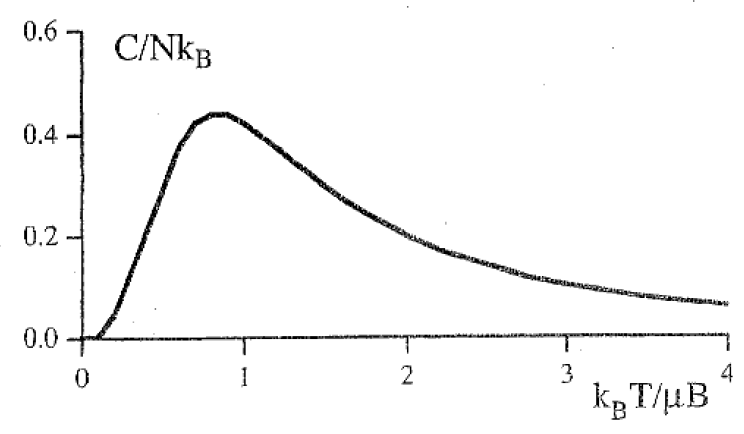
\includegraphics[width=0.6\textwidth]{Immagini/IsingCl.png}
	\vspace{-10pt}
	\caption{}
	\label{fig:isingcp}
	\vspace{-10pt}
\end{figure}

La funzione $ C_P $ tende a $ 0 $ sia per $ T \rightarrow 0 $ che per $ T \rightarrow \infty $. Nel primo caso perché il sistema ha un \textit{gap} finito di energia tra il fondamentale e il primo eccitato (si veda il \cref{chap:crystals}) e quindi i gradi di libertà sono "congelati" a bassa temperatura: non c'è abbastanza energia termica per accedere all'eccitazione unitaria. Nel secondo caso pure la capacità termica si annulla, ma accade perché il sistema è completamente \textit{randomizzato}, per cui le popolazioni nei due stati sono già uguali, e un ulteriore aumento della temperatura non porta a una sostanziale variazione delle popolazioni, e quindi dell'energia.

Il massimo della funzione si ha per $ \mu B / \kt \simeq 1.2 $.

\paragraph{Entropia} L'entropia può essere calcolata a partire dalla funzione di partizione:
\begin{equation*}
S = \frac{E - F}{T} = N k_B \log Z_1 + N \kt \derivative{\log Z_1}{T} = N k_B \log 2 + N k_B \log \cosh(\frac{\mu B}{\kt}) - N K_B \left(\frac{\mu B}{\kt}\right) \tanh(\frac{\mu B}{\kt})
\end{equation*}
che ha i seguenti limiti:
\begin{align*}
S &\simeq N k_B \log 2 \qquad (T\rightarrow \infty)\\
S &= N k_B \log 2 + N k_B \log \frac{e^{\frac{\mu B}{\kt}} + e^{-\frac{\mu B}{\kt}}}{2} - N k_B \left(\frac{\mu B}{\kt}\right) \frac{e^{\frac{\mu B}{\kt}} - e^{-\frac{\mu B}{\kt}}}{e^{\frac{\mu B}{\kt}} + e^{-\frac{\mu B}{\kt}}} \rightarrow 0  \qquad (T \rightarrow 0)
\end{align*}

In accordo con il terzo principio l'entropia si annulla per $ T \rightarrow 0 $, mentre per $ T \rightarrow \infty $ il sistema evolve in uno stato con massima entropia, in cui tutte le $ 2^N $ configurazioni totali sono equiprobabili e l'entropia quindi vale:
\begin{equation*}
S = k_B \log 2^N = N k_B \log 2
\end{equation*}
La funzione entropia è mostrata in \cref{fig:isingentropy}.

\begin{figure}[t]
	\centering
	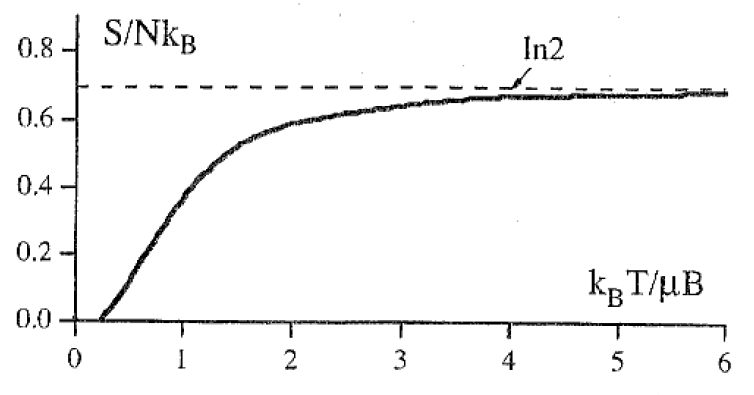
\includegraphics[width=0.6\textwidth]{Immagini/IsingEntropy.png}
	\vspace{-10pt}
	\caption{}
	\label{fig:isingentropy}
	\vspace{-10pt}
\end{figure}

\paragraph{Demagnetizzazione adiabatica} Nella \textit{demagnetizzazione adiabatica} si utilizza questa variazione dell'entropia per raffreddare un campione a temperature molto basse.

Si applicano in sequenza due trasformazioni:
\begin{description}
	\item[isoterma] Partendo da un campo $ B_1 $ si aumenta il campo magnetico fino al valore $ B_2 $, tenendo il sistema a contatto con un bagno termico, in modo che la temperatura sia fissata. In tal modo si genera una diminuzione dell'entropia del sistema.
	\item[adiabatica] Si isola il sistema dal bagno, e quindi esso non scambia calore e mantiene costante la propria entropia. Si riporta quindi il campo magnetico al valore iniziale $ B_1 $.
\end{description}
il processo è mostrato in \cref{fig:demagnad}.
\newline

Applicando le equazioni trovate si ottiene:
\begin{equation*}
T_f = \frac{B_1}{B_2} T_i
\end{equation*}
dove $ T_f, T_i $ sono la temperaura iniziale e finale.

Se il campo magnetico $ B_1 $ si annullasse allora anche la temperatura finale tenderebbe a $ 0 $. Questo però non è realizzabile, infatti è da considerare il campo residuo prodotto dagli altri atomi, che in assenza di campo esterno diventa dominante e pone un limite al minimo raggiungibile per $ B_1 $.

Questo metodo si applica al raffreddamento degli elettroni in un solido, e partendo da temperature $ \sim 1 \kelvin $ si arriva fino a $ \sim 1-10 \milli\kelvin $. Se il metodo è applicato al raffredamento di nuclei, che interagiscono più debolmente, si possono raggiungere anche temperature molto più basse: partendo da $ \sim 10 \milli\kelvin $ si arriva fino a $ \sim 10^{-6} \kelvin $.

\begin{figure}[h]
	\centering
	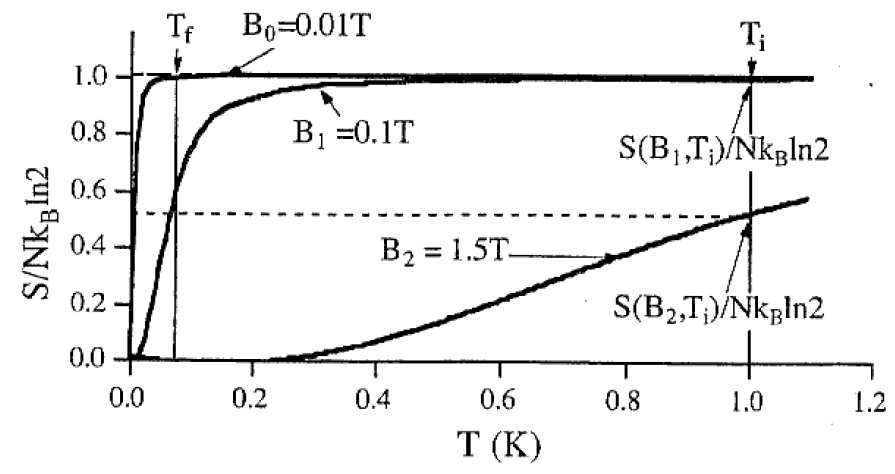
\includegraphics[width=0.6\textwidth]{Immagini/DemagnAdiabatica.png}
	\vspace{-10pt}
	\caption{}
	\label{fig:demagnad}
	\vspace{-10pt}
\end{figure}

\subsubsection{Gas di Fermi}

Per calcolare la magnetizzazione nel caso di un gas di fermioni si può applicare il ragionamento semplicistico degli elettroni al livello di Fermi, affermando che in presenza di un campo magnetico debole (rispetto alla scala dell'energia di Fermi $ \mu B \ll \varepsilon_F $) gli unici elettroni in grado di cambiare stato siano quelli vicino a tale livello.

Si applica quindi il risultato classico a quesi elettroni ottenendo:
\[ M = \left(N \frac{\mu^2 B}{\kt}\right) \frac{\kt}{\mu_{0,F}} = \left(N \frac{\mu^2 B}{\kt}\right) \frac{T}{T_{F}} = N \frac{\mu^2}{\mu_{0,F}} B\]
con $ \mu_{0,F} $ il potenziale chimico dei fermioni a temperatura nulla. 

Da questa espressione risulta quindi che la suscettività magnetica $ \chi = \partial M/\partial B $ di un metallo è indipendente dalla temperatura e più piccola di un fattore $ \kt/\mu_{0,F} $ rispetto al caso classico. Ambedue risultati in accordo con le osservazioni sperimentali.

\begin{figure}[t]
\centering
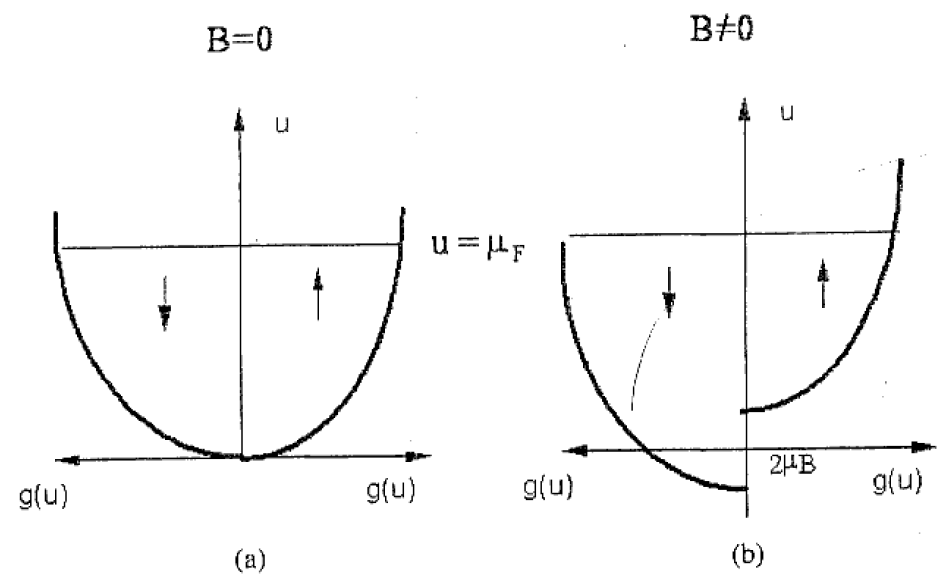
\includegraphics[width=0.8\textwidth]{Immagini/FermiMagnSusc.png}
\vspace{-10pt}
\caption{}
\label{fig:fermimagnsusc}
\vspace{-10pt}
\end{figure}

Si può ottenere un risultato più accurato considerando separatamente le occupazioni degli stati con le due possibili orientazioni di spin (e quindi momento magnetico).
A $ T=0, B=0 $ lo spin agisce solo come un'ulteriore degenerazione, e gli stati sono simmetricamente pieni rispetto all'orientazione, mentre se il campo magnetico è $ B\ne 0 $ l'effetto è quello di sommare un energia $ \mu B $ a tutti gli stati in una configurazione, e sottrarla nell'altra. Quant descritto è mostrato in \cref{fig:fermimagnsusc} (la quantità $ g(u) $ indicata in figura è la densità di stati, che solitamente è stata indicata con $ \rho(\varepsilon) $ in queste dispense).

A bassa temperatura i fermioni riempiono prima i livelli a più bassa energia, per cui la magnetizzazione si potrebbe determinare integrando il numero di elettroni paralleli (quelli che si trovano a energia più bassa dopo l'accensione del campo) in più rispetto a quelli antiparalleli, e moltiplicando per il momento magnetico.
Supponendo che al livello raggiunto dagli elettroni, cioé l'energia di Fermi $ \mu_F $, la funzione $ \rho(\varepsilon) $ sia approssimativamente costante per variazioni dell'ordine di $ \mu B $, si può stimare l'integrale con un rettangolo, la cui base è $ 2 \mu B $ e l'altezza è pari alla densità di stati $ \rho(\varepsilon)/2 $\footnote{Il fattore $ 1/2 $ compare perché nella densità complessiva è contata anche la doppia degenerazione di spin, mentre qui si sta considerando solo uno stato di spin.}:
\[ \Delta N = 2 \mu B \frac{1}{2} \rho(\mu_F) = \frac{3N}{2} \frac{\mu B}{\mu_F}\]
per cui la magnetizzazione risulta:
\[ M = \mu \Delta N = \frac{3N}{2} \frac{\mu^2 B}{\mu_F} \]
e la suscettività:
\[ \chi = \partdev{M}{B} = \frac{3N}{2} \frac{\mu^2}{\mu_F} \]

\subsection{Emissione di elettroni da un metallo}

Per studiare l'emissione degli elettroni da parte di un metallo, sia per eccitazione termica che sotto l'effetto di uno stimolo esterno, si considera che essi all'interno del metallo siano in una buca di potenziale, e si trovino a energia $ - W $, mentre per un elettrone sulla superficie del metallo l'energia potenziale è nulla.

Gli elettroni quindi per fuggire dal metallo devono superare una barriera di potenziale alta $ W $, e quindi devono avere un energia cinetica maggiore o uguale associata alla velocità \textit{perpendicolare} alla superficie.

Questa condizione è necessaria, ma non sufficiente, perché non è trascurabile il coefficiente di riflessione dell'interfaccia, per cui i risultati trovati coincideranno con i risultati sperimentali a meno di un fattore $ (1 - r) $, con $ r $ il \textit{coefficiente di riflessione} della superficie.

\subsubsection{Effetto termoionico}

Si consideri la superficie d'interfaccia perpendicolare all'asse $ z $. Si ha allora che il \textit{rate} di emissione per unità di superficie, cioè il numero di elettroni emessi per unità di tempo e di superficie, è:
\[ R = \int_{p_z = (2mW)^{1/2}}^{\infty}\int_{p_x = -\infty}^{\infty} \int_{p_y = -\infty}^{\infty} \frac{2p_z \dd p_x \dd p_y \dd p_z}{m \hplanck^3}\frac{1}{e^{\varepsilon - \mu / \kt} + 1} \]
ed esprimendo $ p_x $, $ p_y $ e $ p_z $ attraverso coordinate cilndriche $ (p', \varphi, p_z) $ si ottiene:
\begin{align*}
R &= \frac{2}{\hplanck^3}\int_{p_z = (2mW)^{1/2}}^{\infty} \frac{p_z}{m} \dd p_z \int_{p' = 0}^{\infty} \frac{2\pi p' \dd p'}{\exp[(p'^2/2m) + (p_z^2/2m) - \mu / \kt] + 1} =\\
&= \frac{4\pi \kt}{\hplanck^3} \int_{p_z = (2mW)^{1/2}}^{\infty} p_z \dd p_z \log[1 + \exp((\mu - p_z^2/2m)/\kt)]=\\
&= \frac{4\pi m \kt}{\hplanck^3} \int_{\varepsilon_z = W}^{\infty} \dd \varepsilon_z \log[1 + e^{(\mu - \varepsilon_z)/\kt}]
\end{align*}
Risulta inoltre, a tutte le temperature d'interesse, che $ \varepsilon_z \gg \kt + \mu $, per cui si può approssimare il logaritmo al prim'ordine:
\[ R = \frac{4\pi m \kt}{\hplanck^3} \int_{\varepsilon_z = W}^{\infty} \dd \varepsilon_z e^{(\mu - \varepsilon_z)/\kt} = \frac{4\pi m (\kt)^2}{\hplanck^3} e^{(\mu - W)/\kt} \]
per cui la corrente termoionica è:
\[ J = e R =  \frac{4\pi m e k_B^2}{\hplanck^3} T^2 e^{(\mu - W)/\kt} \]

L'unica cosa ancora incognita è il potenziale chimico $ \mu $, o, più direttamente, la fugacità $ z = e^{\mu/\kt} $. Questa è determinata dalla statistica, perciò:
\begin{itemize}
	\item per particelle classiche la fugacità è data da (vedi \cref{sec:idgas}):
	\[ z = e^{\mu/\kt} = \frac{n \Lambda^3}{g} = \frac{n \hplanck^3}{2(2\pi m \kt)^{3/2}} \]
	dove $ \Lambda $ è la lunghezza d'onda termica di De Broglie e $ g $ e un peso che deriva dalla struttura interna (ad esempio lo spin)\footnote{Il peso $ g $ deriva dalla degenerazione di spin presente nella densità di stati $ \rho(\varepsilon) $, anche se nella formula in \cref{sec:idgas} è assente perché si ignoravano i gradi di libertà di spin.}, pari a $ 2 $ in questo caso. La corrente è quindi:
	\[  J_{\text{class}} = ne \left(\frac{k_B}{2\pi m}\right)^{1/2} T^{1/2} e^{-\phi/\kt} \quad (\phi = W)\]
	\item mentre 
	per il gas di Fermi altamente degenere si ha $ \mu \simeq \mu_0 = \varepsilon_F $, e si ottiene per la corrente:
	\[  J_{F.D.} =  \frac{4\pi m e k_B^2}{\hplanck^3} T^2 e^{-\phi/\kt} \quad (\phi = W - \varepsilon_F)\]
\end{itemize}

\subsubsection{Effetto fotoelettrico}

Il problema è simile al precedente effetto termoionico, ma la differenza sostanziale è il contributo energetico di un agente esterno: i fotoni.

Si cerca la corrente prodotta da quegli elettroni che vengono emessi dal metallo in seguito all'assorbimento di un fotone. La condizione che essi devono soddisfare è:
\[ (p_z^2 / 2m) + h \nu > W \] dove $ \nu $ è la frequenza della radiazione incidente.

Procedendo come nel caso precedente si trova:
\[ R = \frac{4\pi m \kt}{\hplanck^3} \int_{\varepsilon_z = W - h\nu}^{\infty} \dd \varepsilon_z \log[1 + e^{(\mu - \varepsilon_z)/\kt}]  \]

In generale non è più possibile in questo caso approssimare il logartimo come nella sezione predente. Si opera quindi un cambiamento di variabile, introducendo $ x $.
\begin{align*}
x &= (\varepsilon_z - W + h\nu)/\kt\\
R &= \frac{4\pi m (\kt)^2}{\hplanck^3} \int_{0}^{\infty} \dd x \log \left[1 + \exp(\frac{h(\nu - \nu{_0})}{\kt} - x)\right] \\
&\text{con} \qquad h\nu_0 = W -\mu \simeq W - \varepsilon_F = \phi
\end{align*}
la quantità $ \phi $ è quella definita nell'ambito dell'effetto termoionico, mentre $ \nu_0 $ è la \textit{frequenza di soglia} per l'effetto fotoelettrico, quella in risonanza col gap di energia fra gli elettroni nel metallo e quelli sulla superficie.

La densità di corrente di emissione fotoelettrica è quindi:
\begin{align*}
J &= \frac{4\pi m e k_B^2}{\hplanck^3} T^2 \int_{0}^{\infty} \dd x \log( 1 + e^{\delta -x}) = \frac{4\pi m e k_B^2}{\hplanck^3} T^2 \int_{0}^{\infty} \frac{x \dd x}{e^{x-\delta}+1} \\
&\text{con} \qquad \delta = h(\nu - \nu_0)/\kt
\end{align*}
dove la seconda uguaglianza nella prima equazione è ottenuta tramite integrazione per parti.

Si possono studiare i casi di valori limite per le frequenze dei fotoni incidenti:
\begin{itemize}
	\item per $ h(\nu - \nu_0) \gg \kt $ si ha $ e^\delta \gg 1 $ e si può calcolare:
		\[ \int_{0}^{\infty} \frac{x \dd x}{e^{x-\delta}+1} \simeq \delta^2/2 \]
		per cui la corrente fotoelettrica diventa:
		\[ J \simeq \frac{me}{\hbar} (\nu - \nu_0)^2\]
		
		Si ha quindi che se l'energia dei fotoni incidenti in eccesso supera di molto l'energia termica la temperatura diventa irrilevante nel processo di emissione.
	\item per $ h(\nu_0 - \nu) \gg \kt $ si ha $ e^{-\delta} \gg 1 $ per cui l'$ 1 $ al denominatore diventa trascurabile:
		\[ \int_{0}^{\infty} \frac{x \dd x}{e^{x-\delta}+1} \simeq e^\delta \int_{0}^{\infty} x e^{-x} \dd x = e^\delta\]
		da cui si ottiene per la corrente:
		\[ J = \frac{4\pi m e k_B^2}{\hplanck^3} T^2 e^{(h\nu - \phi)/\kt}\]
		che è esattamente con l'effetto termoionico, e l'unica conseguenza dei fotoni incidenti è abbassare leggermente il livello della barriera.
	\item per $ \nu = \nu_0 $ si ha $ \delta = 0 $ e si può calcolare:
		\[ \int_{0}^{\infty} \frac{x \dd x}{e^{x}+1} = \frac{\pi^2}{12} \]
		per cui si ottiene la corrente:
		\[ J = \frac{m e k_B^2}{24 \hbar^3} T^2 \]
\end{itemize}

Il fatto che si ottenga una fotocorrente finita anche per fotoni al di sotto della soglia imposta dalla barriera di potenziale è del tutto naturale: quella fotocorrente è generata dagli elettroni della coda termica della distribuzione, per cui i fotoni incidenti vanno a colmare il gap fra quella energia e quella necessaria per la fuga.
Essendo però elettroni appartenenti alle code la fotocorrente sarà esponenzialmente smorzata per barriere sempre più alte, poiché è il numero di elettroni della coda che è esponenzialmente smorzato.

Quest'ultima osservazione non è altro che un modo per reinterpretare il risultato ottenuto al secondo punto \footnote{Abbassare la barriera e poi considerare l'effetto termoionico o considerare direttamente gli elettroni ad alta energia termica e farci incidere i fotoni è la stessa cosa}.


\section{Bibliografia}

Il contenuto di questo capitolo è quasi interamente ispirato al secondo capitolo di \textit{D.L. Goodstein - States of Matter}. La struttura è esattamente la stessa, sono state omesse alcune parti riguardo alle proprietà termodinamiche del gas ideale già studiate nel \cref{chap:termstat} e alcuni argomenti relativi ai condensati non trattati a lezione, ma comunque abbondantemente citati qui per completezza.

La sezione sugli elettroni contiene un certo numero di argomenti tratti da \textit{E. Arimondo - Lezioni di Struttura della Materia}, cioè le dispense del corso tenuto dal prof. Arimondo all'università di Pisa, lo stesso corso cui si riferiscono queste dispense, e due argomenti (effetto termoionico e fotoelettrico) tratti da \textit{R. K. Pathria, P. D. Beale - Statistical Mechanics}.

Seguire più libri porta qualche incongruenza nella notazione. Le variabili usate sono di volta in volta specificate, per cui non c'è ambiguità sul loro significato, però non è garantito che fra sezioni diverse la notazione rimanga la stessa. Spesso è stato preferito riportare direttamente la notazione dei libri usati per limitare gli errori di battitura (se qualcuno volesse normalizzare la notazione è il benvenuto, per cui prenda il \code{tex} e corregga, e se vuole invii una copia corretta all'autore, all'indirizzo: \href{mailto:candido.ale@gmail.com}{candido.ale@gmail.com}).

\vfill

\pagebreak

\section{Schema del capitolo}

\begin{itemize}
	\item Gas Ideale
	\begin{itemize}
		\item numero di particelle $ N $
		\item potenziale di Gibbs $ G $
		\item $ F_{gc} - F_c $, grancanonico - canonico
	\end{itemize}
	\item Statistiche quantistiche
	\item Gas perfetto poco degenere
	\begin{itemize}
		\item $ \Omega $
		\item Interazione efficace
	\end{itemize}
	\item Gas di Fermi
	\begin{itemize}
		\item Energia di Fermi $ \varepsilon_F $
		\item Energia media
		\item Obiezioni alla conduzione
		\item Granpotenziale
		\item Capacità termiche
	\end{itemize}
	\item Gas di Bose
	\begin{itemize}
		\item Temperatura critica - Densità critica
		\item Proprietà di un condensato
	\end{itemize}
	\item Elettroni nei metalli
	\begin{itemize}
		\item Conduzione
		\begin{itemize}
			\item Drude
			\item Drude quantistico
			\item trasporto di Boltzmann
		\end{itemize}
		\item Campi magnetici
		\begin{itemize}
			\item classico
			\item quantistico (2 modi)
		\end{itemize}
		\item Emissione
		\begin{itemize}
			\item termoionico
			\item fotoelettrico
		\end{itemize}
	\end{itemize}
\end{itemize}
